% =====================================================================
%  CO3133 - Deep Learning and Its Applications - Semester 261
%  Assignment 3 - M3 final report - Group G-roundhog
%  Compiles with pdfLaTeX (needs vntex for the Vietnamese names; on Overleaf by default)
%  or with XeLaTeX / LuaLaTeX:  latexmk -pdf main.tex
% =====================================================================
\documentclass[11pt,a4paper]{article}

\usepackage{iftex}
\ifPDFTeX
  \usepackage[utf8]{inputenc}
  \usepackage[T5]{fontenc}
  \usepackage{lmodern}
\else
  \usepackage{fontspec}
\fi

\usepackage[margin=2.5cm]{geometry}
\usepackage{amsmath,amssymb,mathtools,bm}
\usepackage{booktabs,tabularx,array,multirow}
\usepackage{graphicx}
\graphicspath{{figures/}}
\usepackage{subcaption}
\usepackage{float}
\usepackage{tikz}
\usetikzlibrary{positioning,arrows.meta}
\usepackage{xcolor}
\usepackage{microtype}
\usepackage{xurl}
\usepackage[numbers,sort&compress]{natbib}
\usepackage[hidelinks]{hyperref}
\usepackage[capitalise,noabbrev]{cleveref}

\setcounter{secnumdepth}{3}
\setlength{\emergencystretch}{3em}   % long \texttt names: stretch spaces instead of overflowing
\newcolumntype{Y}{>{\raggedright\arraybackslash}X}
\newcommand{\R}{\mathbb{R}}
\newcommand{\cls}[1]{\texttt{#1}}
\newcommand{\pending}[1]{\textcolor{orange!80!black}{\textit{[#1]}}}
\DeclareMathOperator*{\argmax}{arg\,max}
\DeclareMathOperator{\LN}{LN}
\DeclareMathOperator{\CE}{CE}

\begin{document}
\begin{center}
\vspace{2em}
\begin{Large}
VietNam National University Ho Chi Minh City\\
Ho Chi Minh City University of Technology\\
Faculty of Computer Science and Engineering

\vspace{6em}

\includegraphics[width=0.25\linewidth]{figures/HCMUT.png} \\
\vspace{8em}
\textbf{
Deep Learning and its applications (CO3133)\\
Assignment 3 Draft Report (Milestone M2)\\
\Huge Multimodal Recipe Classification\\[0.2em]
\LARGE from Web Images and Page Titles\\
}
\vspace{4em}
\textbf{CC01 Group G-roundhog}
\begin{table}[h!]
  \centering
    \begin{tabular}{ll}
    \textbf{Instructor} & \\
    Lê Thành Sách  & \\
    & \\
    \textbf{Student Name} & \textbf{Student ID} \\
    Phan Ba Thanh & 2353084 \\
    Tran Cong Hoang Phuoc & 2352966 \\
    \end{tabular}
\end{table}

\end{Large}
\vspace*{\fill}
\end{center}
\clearpage

\tableofcontents
\clearpage

% =====================================================================
%  Summary of the final report
% =====================================================================
\section*{Summary}
\addcontentsline{toc}{section}{Summary}

This is the final report of Assignment~3 (milestone M3, specification section~6.13: \emph{improved fusion and
ablations complete}). We classify recipe web pages of UPMC Food-101 into 101 dishes from one image and the page
title. The dataset proposal (M1) and the M2 draft were approved by the instructor.

\paragraph{What was built.}
\begin{itemize}
  \item \textbf{Two unimodal baselines:} UA, an image model on ResNet-50, and UB, a text model on DistilBERT.
  \item \textbf{Three fusions:}
        \begin{itemize}
          \item F0, a late fusion of the two softmax outputs;
          \item F1, a concat fusion trained end to end;
          \item F2, the improved fusion. It is a cross-modal transformer over image-region and title tokens, with
                auxiliary unimodal losses and modality dropout.
        \end{itemize}
  \item \textbf{Two text references:} a keyword rule (K0) and TF-IDF with logistic regression (T0).
  \item \textbf{Three ablations of F2:} the auxiliary losses (E1), class names masked in every title (E2) and the
        modality dropout (E4). F2 and its ablations are also tested with each modality removed from part of the
        test set (E-mod).
\end{itemize}
All trained models were run with three seeds. Every decision uses the rule registered in the proposal.

\paragraph{Main findings.}
\begin{enumerate}
  \item \textbf{Fusion helps a lot.} Every fusion is $6$--$7$\,pp of macro-F1 above the best unimodal model
        (UB, $86.8\%$).
  \item \textbf{F2 beats F1 but not F0.} F2 reaches $93.53\pm0.07\%$ macro-F1. It is significantly better than
        F1 ($+0.73$\,pp) and as good as F0 ($-0.33$\,pp, not significant). F2 is also the best-calibrated model.
  \item \textbf{Class names drive the result.} Masking them drops the text-only model from $86.8$ to $43.7\%$.
        On masked titles, F2 is the best fusion: $+2.5$\,pp over F0 and $+0.9$\,pp over F1, both significant.
  \item \textbf{The auxiliary losses matter, the modality dropout only helps with a missing title.}
        \begin{itemize}
          \item Removing the auxiliary losses costs $0.46$\,pp (significant). It also weakens the image branch:
                accuracy without the title falls from $65.3$ to $58.6\%$.
          \item Removing the modality dropout does not change the full-test score. It costs $4.7$\,pp when the
                title is removed.
        \end{itemize}
  \item \textbf{The conflict groups explain the remaining errors.} A manual review of 100 conflict items shows
        two main causes. When only the image model is right, the title is mostly generic ($84\%$); fusion fixes
        almost all of these. When only the text model is right, the image mostly looks like another dish ($68\%$).
        The hard case is a title that names another dish: every fusion gets only about half of these right.
\end{enumerate}

\paragraph{Traceability.}
\begin{itemize}
  \item \textbf{Split:} every number comes from the committed split \texttt{data/splits/split.json}.
  \item \textbf{Code:}
        \begin{itemize}
          \item UA, UB and F1 (M2): commit \texttt{cfc509a};
          \item F2, the ablations and T0 (M3): commit \texttt{b51d3fb};
          \item analyses: commit \texttt{850b6bb} and later.
        \end{itemize}
        Each run records its commit in its \texttt{env.json} file, always with a clean working tree.
  \item \textbf{Checkpoints:} the selected checkpoints, with SHA-256 checksums, are linked in the Required Links
        section.
\end{itemize}


\part*{Part 1: Problem and Data Description}
\addcontentsline{toc}{part}{Part 1: Problem and Data Description}
% =====================================================================
%  Part 1: Problem and data description
% =====================================================================
\setcounter{section}{0}
\section{Problem and Data Description}
\label{sec:part1}

\subsection{Problem Formulation}
\label{sec:problem}

Each sample is one \emph{recipe web page} returned by a Google Image search for
``\texttt{<dish> recipe}''~\cite{wang2015recipe}. It provides two modalities that come from the same page:
an RGB image $x^{I}$ and the page title $x^{T}$, a short string. The label $y$ is one of $K=101$ dish classes,
the same classes as Food-101~\cite{bossard2014food} in Assignment~2. A model $f_\theta$ outputs logits in
$\R^{K}$ and is trained with the cross-entropy loss
\begin{equation}
  \mathcal{L}(\theta) = -\frac{1}{N}\sum_{n=1}^{N} \log \operatorname{softmax}\big(f_\theta(x^{I}_n, x^{T}_n)\big)_{y_n}.
\end{equation}
Unimodal models see only $x^{I}$ or only $x^{T}$.

The two modalities carry different evidence, and each fails in its own way. The image shows the
appearance of the dish, but web images include advertisements, collages, ingredient shots and photos shared
by several dishes. The title often names the dish, but it can be generic (``Recipes''), describe a derived
dish (``Apple Pie Moonshine'') or name another class. These cases are the \emph{support} and \emph{conflict}
cases that the specification asks us to analyse (section~6.11).

\subsection{Dataset}
\label{sec:dataset}

We use UPMC Food-101~\cite{wang2015recipe} through the Kaggle mirror \texttt{gianmarco96/upmcfood101}.
It contains $90{,}704$ JPEG images in the official train/test lists ($67{,}988$ / $22{,}716$) and two CSV
files with the \textbf{page title} of each image. The mirror does not contain the full page text that earlier
work used~\cite{kiela2019mmbt}, so our text modality is the title only. We use the data for research only and
do not redistribute images or titles; only code, split id lists and checkpoints are published.

\subsection{Pairs and Validity}
\label{sec:pairs}

The linking entity is the \textbf{web page}. An image and a title form a pair only when they share the file
id \texttt{<label>\_<num>}, the label and the official split; samples are never paired at random. The script
\texttt{scripts/prepare\_data.py} checks the validity criteria of the proposal (\cref{tab:validity}).
A \emph{complete pair} satisfies criteria 1--3. All models are trained, selected and tested on complete pairs.
Items whose title fails criterion~2 form the natural missing-text set.

\begin{table}[H]
  \centering\small
  \caption{Pair-validity criteria and their outcome on the full dataset.}
  \label{tab:validity}
  \begin{tabularx}{\linewidth}{@{}lYl@{}}
    \toprule
    Criterion & Rule & Result \\
    \midrule
    1. Image valid & decodes, shorter side $\ge 64$\,px, pixel standard deviation $> 2$ & $90{,}701$ / $90{,}704$ \\
    2. Text valid  & a title row exists and contains at least one content word ($\ge 3$ letters, not in a fixed list of generic web words such as \emph{recipes}, \emph{easy}, \emph{pinterest}) & $90{,}192$ / $90{,}704$ \\
    3. Same item   & same id, label and official split & all $90{,}688$ titles matched \\
    4. Manual audit & 200 train pairs, 10 from each of 20 random classes & $81.5\%$ valid (\cref{sec:audit}) \\
    \bottomrule
  \end{tabularx}
\end{table}

Of the $512$ items without a valid title, $16$ have no title row at all and $496$ fail the content-word rule.
The most frequent failing titles are ``All Yummy Recipes'', ``Recipes'', ``Recipes on Pinterest'', ``Easy'' and
``Food''. Three images are near-constant placeholders.

\subsection{Exploratory Data Analysis}
\label{sec:eda}

The EDA (\texttt{scripts/eda.py}) covers pair counts, pair quality, missing-modality rates and
modality-specific distributions, as required by section~6.10. \Cref{fig:samples} shows random training pairs.

\begin{figure}[H]
  \centering
  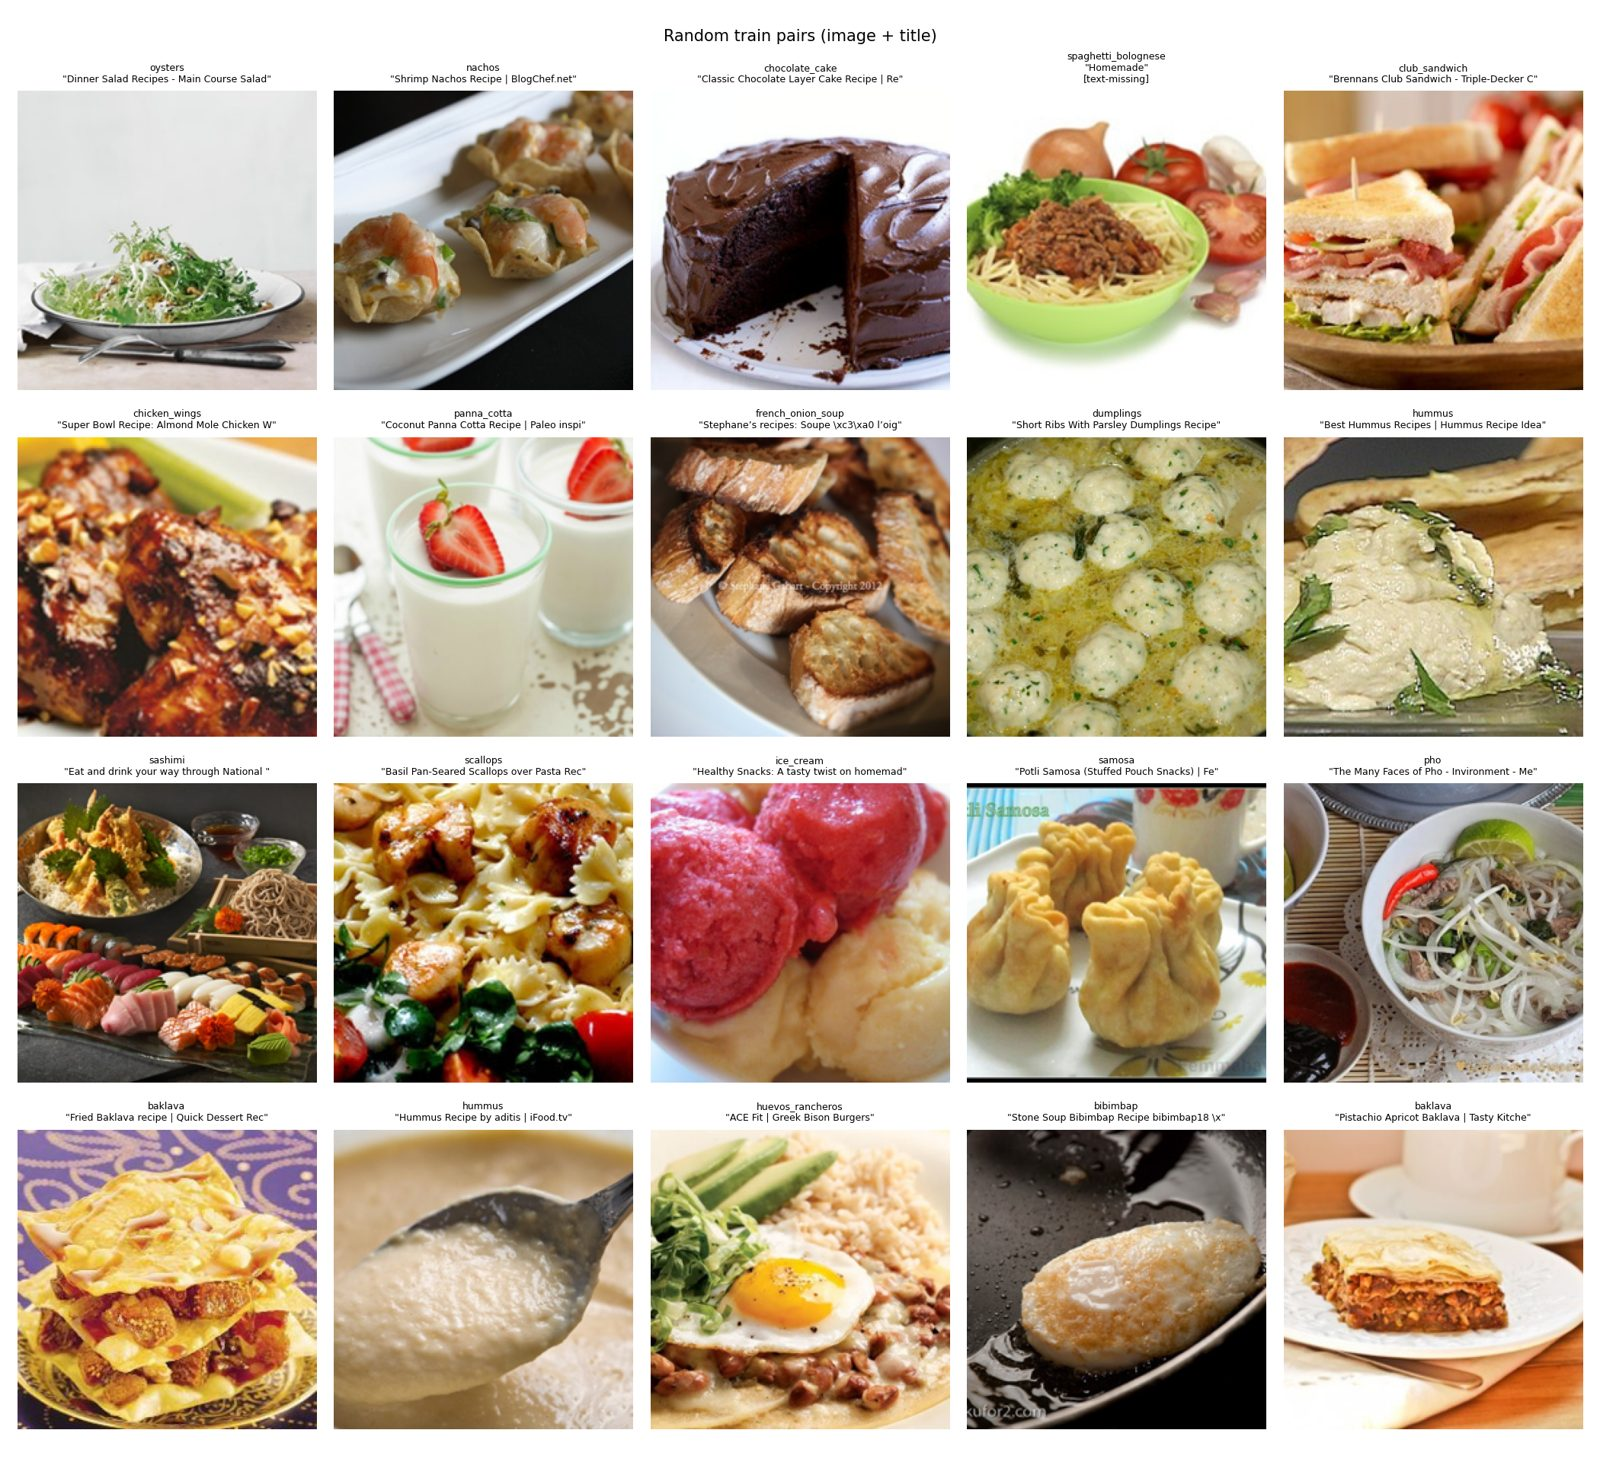
\includegraphics[width=0.95\linewidth]{samples_pairs.jpg}
  \caption{Twenty random training pairs with their class label and title. Titles are noisy web strings: site
  names, generic titles (``Homemade'' fails the validity rule), derived dishes, and pages whose title does not
  describe the image.}
  \label{fig:samples}
\end{figure}

\paragraph{Pair counts and missing modalities.}
\Cref{tab:counts} gives the counts per split. Missing modalities are rare: about $0.6\%$ of the items have an
uninformative title, and only three images are invalid. The classes are mildly imbalanced (largest/smallest
class $1.21$ in train), so macro-F1 is the primary metric. The highest text-missing rates per class are
\cls{hot\_dog} ($5.5\%$) and \cls{breakfast\_burrito} ($3.5\%$).

\begin{table}[H]
  \centering\small
  \caption{Items per split after the pair checks.}
  \label{tab:counts}
  \begin{tabular}{@{}lrrrrrr@{}}
    \toprule
    Split & Items & Complete pairs & Text-missing & Image-missing & Train duplicate & Cross-label cluster \\
    \midrule
    train & $63{,}128$ & $\mathbf{62{,}771}$ & $355$ & $2$ & -- & $869$ \\
    val   & $4{,}860$  & $\mathbf{4{,}824}$  & $36$  & $0$ & -- & $75$ \\
    test  & $22{,}716$ & $\mathbf{22{,}594}$ & $121$ & $1$ & $3{,}290$ ($14.5\%$) & $296$ \\
    \bottomrule
  \end{tabular}
\end{table}

\paragraph{Label information in the title.}
The search query leaked the class name into most titles. We match titles against a class-name lexicon
(names, singular and plural forms, and 82 hand-written synonyms for 50 classes, fixed from the class list and
train titles only). \Cref{tab:mention} summarises the results. A keyword rule that predicts the most-mentioned
class (K0) already reaches $76.8\%$ test accuracy without any learning. The share of titles that name their
own class ranges from $7\%$ (\cls{hot\_dog}) and $30\%$ (\cls{beef\_tartare}) to $97.5\%$ (\cls{pancakes}),
see \cref{fig:mention}.

\begin{table}[H]
  \centering\small
  \caption{Class names in titles (complete pairs).}
  \label{tab:mention}
  \begin{tabular}{@{}lrrrrr@{}}
    \toprule
    Split & Own class, exact & Own class, lexicon & Another class only & No class & K0 accuracy \\
    \midrule
    train & $72.3\%$ & $78.8\%$ & $1.0\%$ & $20.2\%$ & $76.9\%$ \\
    test  & $72.4\%$ & $78.8\%$ & $0.9\%$ & $20.2\%$ & $76.8\%$ \\
    \bottomrule
  \end{tabular}
\end{table}

\begin{figure}[H]
  \centering
  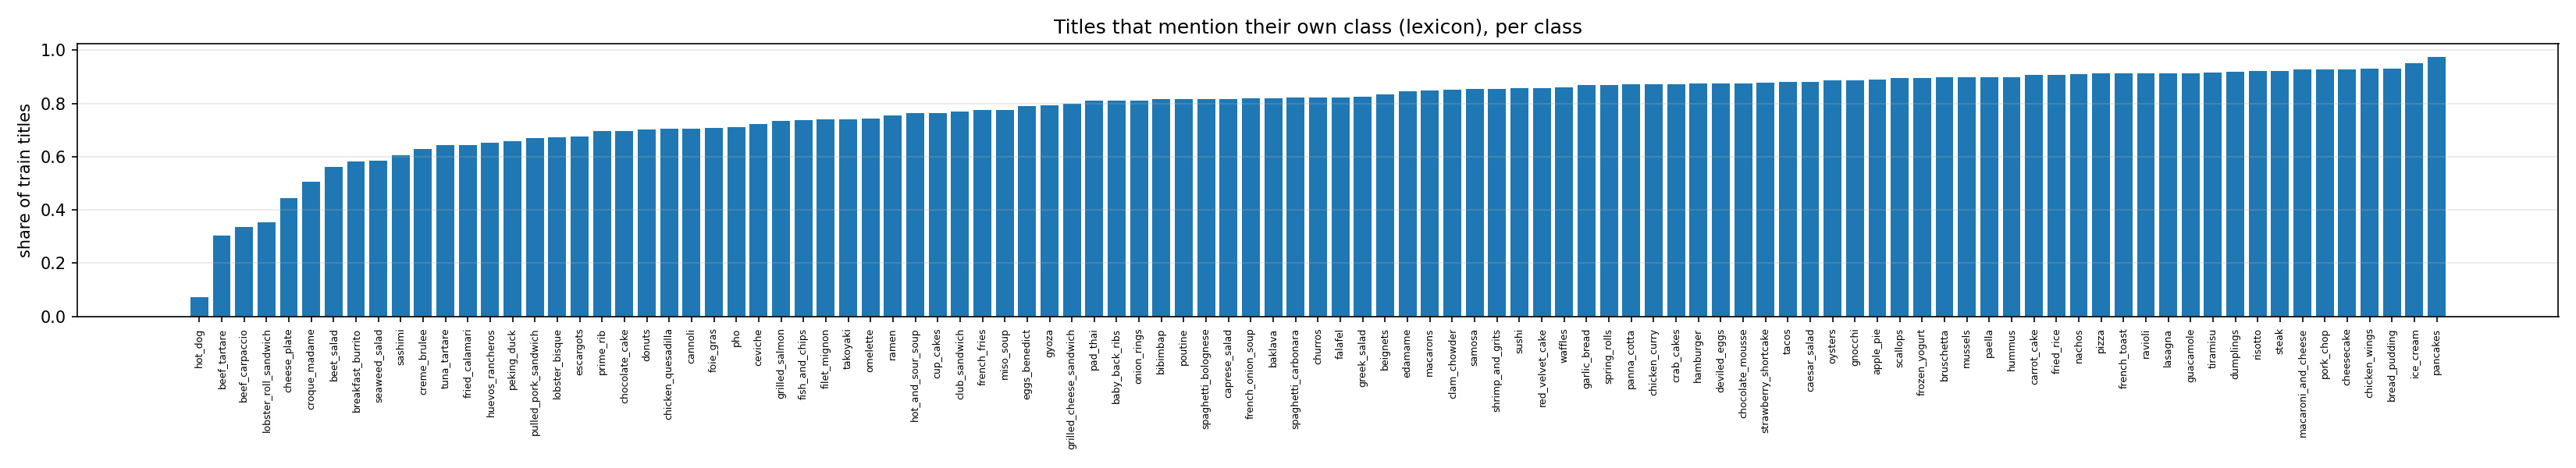
\includegraphics[width=\linewidth]{class_name_mention_per_class.png}
  \caption{Share of train titles that mention their own class, per class (sorted).}
  \label{fig:mention}
\end{figure}

\paragraph{Text distributions.}
Titles are short: the median is $7$ words and $13$ DistilBERT tokens, the 99th percentile $39$ tokens. Only
$126$ titles ($0.14\%$) exceed the $64$-token limit (\cref{fig:text}). The train vocabulary has $29{,}847$
lower-cased words.
\begin{itemize}
  \item \textbf{Site names.} $64\%$ of the titles end with a site segment (``| Taste of Home'', ``on Pinterest'').
        For the $96$ sites with at least $50$ train items, the majority class covers only $16\%$ of a site's
        items on average, so the site name alone is a weak class cue.
  \item \textbf{Encoding errors.} Some titles contain literally escaped UTF-8 bytes
        (``Soupe \textbackslash xc3\textbackslash xa0 l'oig'') or JSON-like brackets. These are crawl errors
        that we keep as they are.
\end{itemize}

\begin{figure}[H]
  \centering
  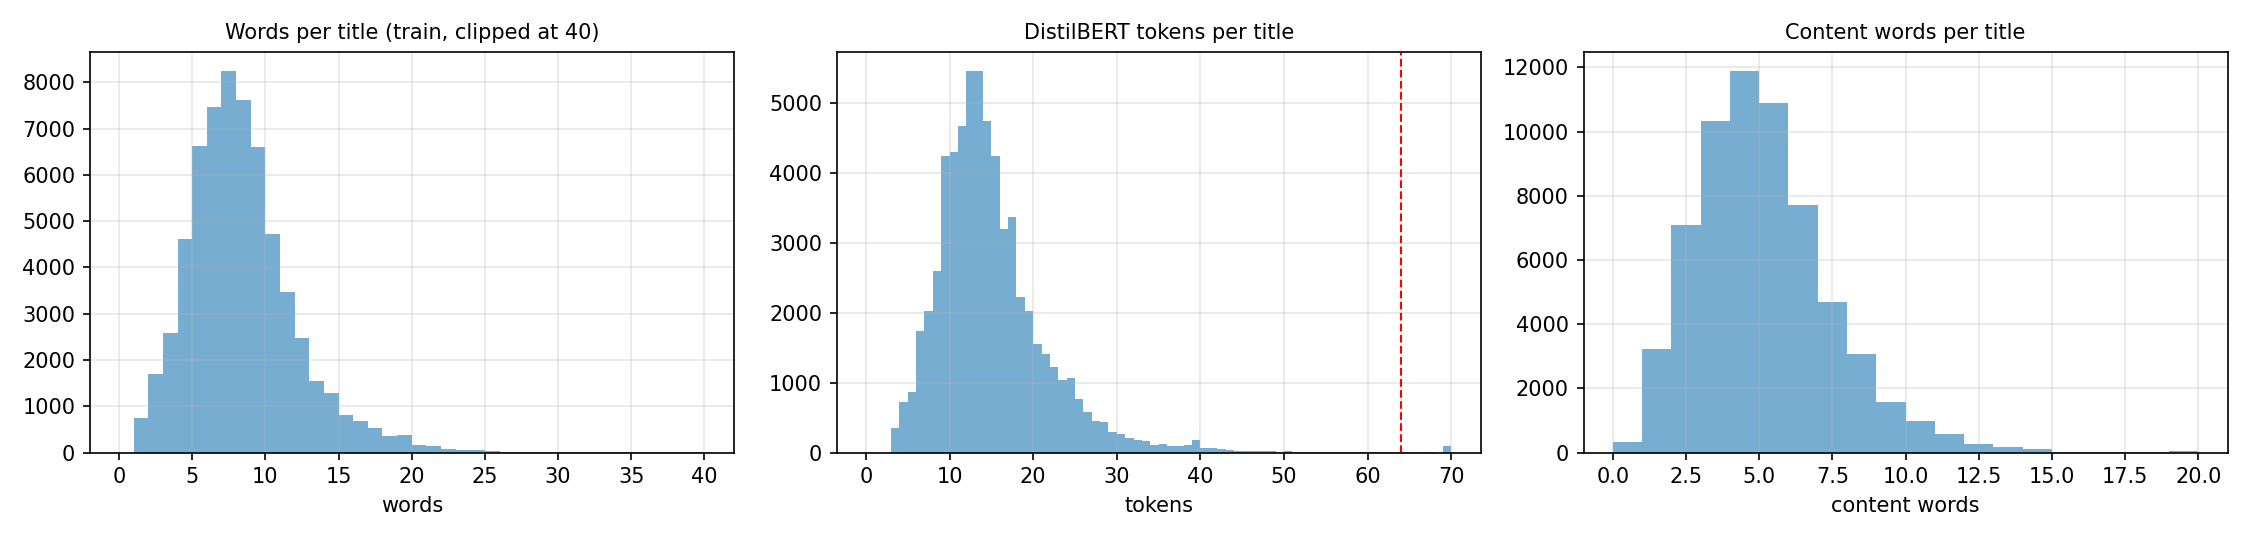
\includegraphics[width=\linewidth]{text_lengths.png}
  \caption{Words, DistilBERT tokens and content words per train title. The red line marks the 64-token limit.}
  \label{fig:text}
\end{figure}

\paragraph{Image distributions.}
The images are web photos of varied geometry (\cref{fig:images}).
\begin{itemize}
  \item Shorter side: median $387$\,px, range $120$--$900$\,px.
  \item Aspect ratio: median $1.33$, range $0.09$--$8.73$. The extreme values are banners and collages.
  \item The training mean colour $[0.628, 0.529, 0.422]$ is brighter than ImageNet's $[0.485, 0.456, 0.406]$
        because many recipe sites use white backgrounds. The pretrained encoders still use the ImageNet
        statistics they were trained with.
\end{itemize}
We store a copy resized to a shorter side of $256$\,px, which keeps all the detail used at $224$\,px.

\begin{figure}[H]
  \centering
  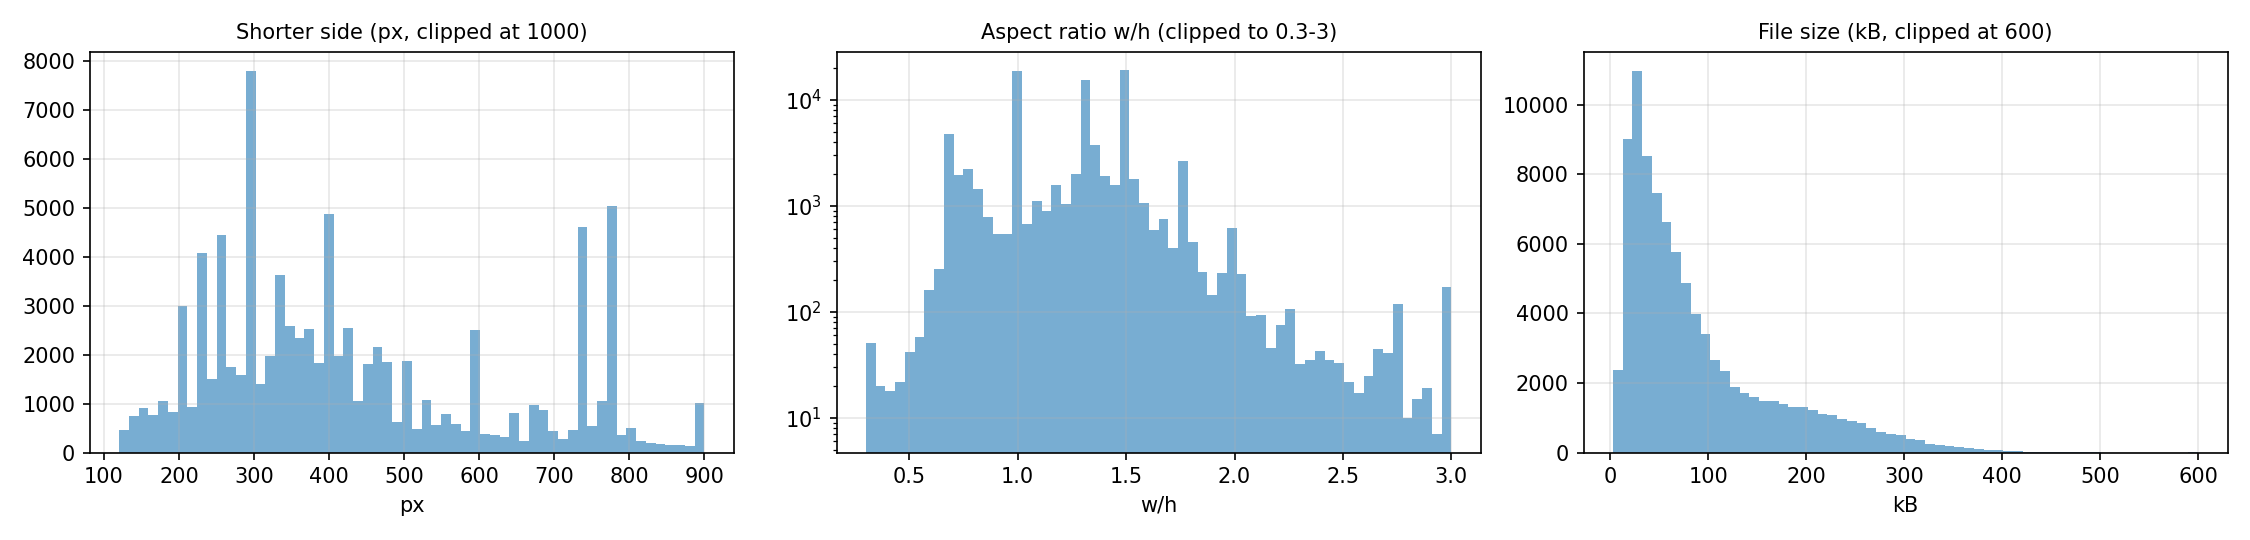
\includegraphics[width=\linewidth]{image_stats.png}
  \caption{Shorter side, aspect ratio and file size of all images.}
  \label{fig:images}
\end{figure}

\paragraph{Duplicates.}
We link two items when their files are identical (md5) or when their 64-bit perceptual hashes~\cite{zauner2010phash}
differ by at most $4$ bits.
\begin{itemize}
  \item There are $3{,}597$ md5 links and $12{,}663$ pHash pairs. Their connected components form $7{,}201$
        clusters with at least two items ($16{,}498$ items; the largest cluster has $16$).
  \item $524$ clusters carry two or more labels (\cref{fig:dups}), which is label noise built into the crawl.
  \item $3{,}290$ test items ($14.5\%$) are linked to an image in the official train list.
  \item Independently of the images, $10{,}859$ normalised titles occur more than once, $4{,}873$ of them in
        both official lists.
\end{itemize}

\begin{figure}[H]
  \centering
  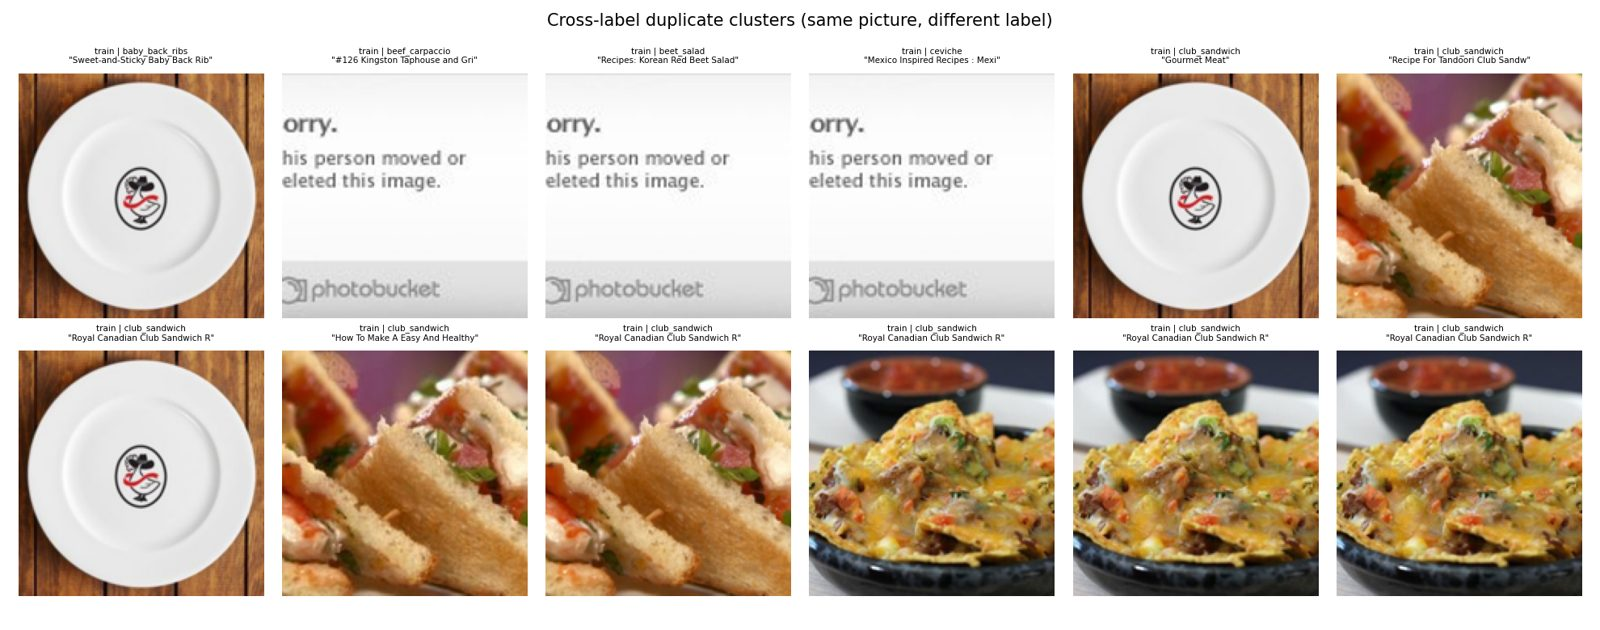
\includegraphics[width=0.9\linewidth]{duplicates_cross_label.jpg}
  \caption{Cross-label duplicate clusters: the same picture appears under different classes.}
  \label{fig:dups}
\end{figure}

\subsection{Pair Audit}
\label{sec:audit}

Ten random train pairs were drawn from each of 20 random classes (seed $42$) and labelled by hand with
\texttt{scripts/audit\_pairs.py}: Phan Bá Thanh labelled pairs 1--100 and Trần Công Hoàng Phước pairs 101--200.
Each pair is classified as \emph{valid}, \emph{image unrelated}, \emph{text unrelated}, \emph{both unrelated},
or \emph{wrong label} (image and title agree with each other but not with the class). Rates are reported with
Wilson $95\%$ confidence intervals~\cite{wilson1927}.

\begin{table}[H]
  \centering\small
  \caption{Manual audit of 200 train pairs (\texttt{data/audit/pair\_audit.csv}).}
  \label{tab:audit}
  \begin{tabular}{@{}lrrl@{}}
    \toprule
    Verdict & Count & Rate & Wilson 95\% CI \\
    \midrule
    valid           & $163$ & $\mathbf{81.5\%}$ & $75.5$--$86.3\%$ \\
    image unrelated & $16$  & $8.0\%$  & $5.0$--$12.6\%$ \\
    text unrelated  & $17$  & $8.5\%$  & $5.4$--$13.2\%$ \\
    both unrelated  & $3$   & $1.5\%$  & $0.5$--$4.3\%$ \\
    wrong label     & $1$   & $0.5\%$  & $0.1$--$2.8\%$ \\
    \midrule
    \textit{image uninformative (image + both)} & $19$ & $9.5\%$  & $6.2$--$14.4\%$ \\
    \textit{title uninformative (text + both)}  & $20$ & $10.0\%$ & $6.6$--$14.9\%$ \\
    \bottomrule
  \end{tabular}
\end{table}

\begin{itemize}
  \item \textbf{One pair in five is noisy, and usually in one modality only.} Only $1.5\%$ of the pairs are
        unrelated in both modalities. When one side is uninformative, the other usually still carries the class.
        These pairs are the raw material of the conflict groups (\cref{sec:support}).
  \item \textbf{The noise is concentrated in a few classes:}
        \begin{itemize}
          \item \cls{peking\_duck}: 5 of its 10 images are unrelated;
          \item \cls{grilled\_salmon}: 5 of its 10 titles are unrelated;
          \item \cls{hot\_and\_sour\_soup}: 4 of its 10 titles are unrelated;
          \item seven of the 20 classes have no noisy pair at all.
        \end{itemize}
  \item \textbf{The automatic text rule is lenient.} Criterion~2 flags only 2 of the 20 titles judged
        uninformative. It catches empty or generic titles, but not the titles of other pages or recipes.
        The real share of uninformative titles is therefore about $10\%$, not the $0.6\%$ text-missing rate of
        \cref{tab:counts}, and the natural missing-text set understates real missingness. A missing class name is
        a strong but not sufficient signal of a useless title: 19 of the 20 uninformative titles do not mention
        the class, against 19 of the 180 informative ones.
  \item \textbf{Wrong labels are rare ($0.5\%$).} The ETHZ Food-101 train set of Assignment~2 had $6.7\%$. Here the
        image and the title come from the same query page, so they rarely agree on a different dish. The
        cross-label duplicate clusters are the main source of label noise.
  \item \textbf{Limitations.} Each pair was judged by one rater, so there is no inter-rater agreement. The sample
        covers 20 of the 101 classes.
\end{itemize}

\subsection{Data Splitting and Leakage Prevention}
\label{sec:split}

\begin{itemize}
  \item \textbf{Split unit.} The item (one web page) is the split unit, so an image and its title can never fall into
        different splits (specification, section~6.4).
  \item \textbf{Validation.} The official train list is split by
        \texttt{StratifiedGroupKFold}~\cite{pedregosa2011sklearn} with $14 = \mathrm{round}(67{,}988/5{,}000)$ folds,
        shuffling and seed $42$. Class is the stratum and the image-duplicate cluster is the group; fold~0 is the
        validation set ($4{,}860$ items). The code asserts that no cluster is shared by train and validation.
  \item \textbf{Test.} The official test list is kept unchanged for comparability, so test items with a train
        duplicate cannot be moved. Instead, every test metric is reported again on a \textbf{dedup} subset
        ($19{,}270$ complete pairs without a train-linked image and without cross-label clusters).
  \item \textbf{Title leakage (found in M2).} $39.4\%$ of the complete test pairs ($8{,}893$) have a normalised
        title that also occurs in train or validation. Either several images of one page were split across the
        official lists, or the title is generic. The image clusters cannot see these links, so we add a third
        view: the $13{,}701$ \textbf{title-unseen} test items (\cref{sec:leakage}).
  \item \textbf{Train-only statistics.} The lexicon and the generic-word list use train information only; the image
        models use the ImageNet statistics.
  \item \textbf{Committed files.} The split is committed as \texttt{data/splits/\{train,val,test\}.csv} with
        truncated SHA-256 fingerprints in \texttt{split.json}. Every run checks these fingerprints.
\end{itemize}


\part*{Part 2: Methodology}
\addcontentsline{toc}{part}{Part 2: Methodology}
% =====================================================================
%  Part 2: Methodology
% =====================================================================
\section{Methodology}
\label{sec:method}

\subsection{Pipeline}

\begin{figure}[H]
  \centering
  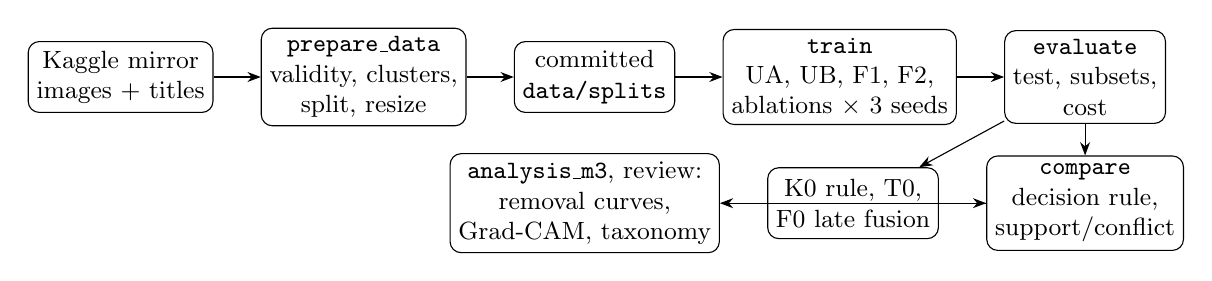
\begin{tikzpicture}[node distance=4mm and 6mm, every node/.style={font=\small},
      box/.style={draw, rounded corners, align=center, minimum height=9mm, inner sep=3pt},
      >={Stealth}]
    \node[box] (raw) {Kaggle mirror\\images + titles};
    \node[box, right=of raw] (prep) {\texttt{prepare\_data}\\validity, clusters,\\split, resize};
    \node[box, right=of prep] (split) {committed\\\texttt{data/splits}};
    \node[box, right=of split] (train) {\texttt{train}\\UA, UB, F1, F2,\\ablations $\times$ 3 seeds};
    \node[box, right=of train] (eval) {\texttt{evaluate}\\test, subsets,\\cost};
    \node[box, below=of eval] (cmp) {\texttt{compare}\\decision rule,\\support/conflict};
    \node[box, left=of cmp] (ref) {K0 rule, T0,\\F0 late fusion};
    \node[box, left=of ref] (ana) {\texttt{analysis\_m3}, review:\\removal curves,\\Grad-CAM, taxonomy};
    \draw[->] (raw) -- (prep); \draw[->] (prep) -- (split); \draw[->] (split) -- (train);
    \draw[->] (train) -- (eval); \draw[->] (eval) -- (cmp); \draw[->] (eval) -- (ref); \draw[->] (ref) -- (cmp); \draw[->] (cmp) -- (ana);
  \end{tikzpicture}
  \caption{Pipeline. Every step is a script in the repository; every run stores its configuration, environment,
  log, history, selected checkpoint and test outputs.}
  \label{fig:pipeline}
\end{figure}

\subsection{Modality-Specific Encoders}
\label{sec:encoders}

\paragraph{Image encoder.}
We use ResNet-50~\cite{he2016resnet} with the torchvision ImageNet-1k weights \texttt{IMAGENET1K\_V2}, the same
backbone as P1 in Assignment~2, without its classification layer. A $224\times224$ crop gives the pooled feature
$\mathbf{u} = g_I(x^{I}) \in \R^{2048}$.

\paragraph{Text encoder.}
We use DistilBERT-base-uncased~\cite{sanh2019distilbert}, a 6-layer distilled BERT~\cite{devlin2019bert} with
hidden size $768$. Titles are HTML-unescaped and tokenised with its uncased WordPiece tokenizer (at most 64
tokens). Each batch is trimmed to the length of its longest title. The final hidden state of the
\texttt{[CLS]} token gives $\mathbf{v} = g_T(x^{T}) \in \R^{768}$.

\paragraph{Alignment.}
The two modalities are aligned at the item level through the shared page id. There is no word-to-region
annotation. F2 learns a soft token-level alignment with cross-modal attention between image regions and title
tokens (\cref{sec:f2}); the other models only align the two modalities at the item level.

\subsection{Models}
\label{sec:models}

\begin{table}[H]
  \centering\small
  \caption{Models. The parameter counts are printed by the code.}
  \label{tab:models}
  \begin{tabularx}{\linewidth}{@{}llYr@{}}
    \toprule
    ID & Modalities & Definition & Parameters \\
    \midrule
    K0 & text  & most-mentioned class in the title (lexicon, ties broken by the first mention); otherwise the most frequent train class & 0 \\
    T0 & text  & TF-IDF of word 1--2-grams and character 3--5-grams, multinomial logistic regression~\cite{pedregosa2011sklearn} & $13.6$\,M \\
    UA & image & $\operatorname{Linear}_{2048\to101}(\mathbf{u})$ & $23.71$\,M \\
    UB & text  & $\operatorname{Linear}_{768\to101}(\operatorname{Dropout}_{0.1}(\mathbf{v}))$ & $66.44$\,M \\
    F0 & both  & $\mathbf{p} = w\,\mathbf{p}_{\mathrm{UA}} + (1-w)\,\mathbf{p}_{\mathrm{UB}}$, with $w$ chosen on validation & $0$ extra \\
    F1 & both  & concat fusion, \cref{eq:f1} & $91.89$\,M \\
    F2 & both  & cross-modal transformer fusion with auxiliary losses and modality dropout, \cref{sec:f2} & $97.98$\,M \\
    \bottomrule
  \end{tabularx}
\end{table}

\paragraph{Late fusion (F0).}
F0 averages the softmax outputs of the UA and UB runs of the same seed. The weight is
$w^\star = \argmax_{w \in \{0, 0.05, \dots, 1\}} \mathrm{MacroF1}_{\mathrm{val}}(w)$. The selected weights are
$0.45$, $0.45$ and $0.50$ for seeds 42, 123 and 2026. F0 needs no training, so it is a reference that tells us how
much of the gain of a trained fusion comes from simply combining two good unimodal predictions.

\paragraph{Concat fusion (F1, intermediate fusion).}
Each modality is projected to $d=512$ and normalised. The two vectors are multiplied by availability masks
$m_I, m_T \in \{0,1\}$, concatenated and passed through an MLP:
\begin{equation}
  \label{eq:f1}
  \mathbf{h}_I = m_I \LN(W_I\mathbf{u}), \qquad
  \mathbf{h}_T = m_T \LN(W_T\mathbf{v}), \qquad
  f_{\mathrm{F1}} = W_2\,\operatorname{Dropout}_{0.1}\!\big(\operatorname{GELU}(W_1[\mathbf{h}_I;\mathbf{h}_T])\big),
\end{equation}
with $W_I \in \R^{512\times2048}$, $W_T \in \R^{512\times768}$, $W_1 \in \R^{512\times1024}$ and
$W_2 \in \R^{101\times512}$. The whole model, including both encoders, is trained end to end with one
cross-entropy loss on the fused logits.

\paragraph{Missing-modality handling.}
F1 zero-fills the projected vector of a missing modality ($m=0$). F0 falls back to the available unimodal model.
F1 is trained on complete pairs only, so zero-filling is outside its training distribution. F2 is trained
with missing modalities (modality dropout) and uses learned \texttt{[MISSING]} tokens instead.

\paragraph{Losses.}
UA, UB and F1 each use a single cross-entropy loss. F2 adds per-modality auxiliary losses (\cref{eq:f2loss}),
which are tested in ablation E1.

\subsection{Improved Fusion (F2)}
\label{sec:f2}

The M2 analysis showed that F1 under-uses the image. The title alone fits the training set, so the image branch
inside F1 ends up weaker than the standalone image model. F2 targets this failure with three changes, all fixed in
the proposal before any F2 run: token-level cross-modal attention, auxiliary unimodal losses, and modality dropout.

\begin{figure}[H]
  \centering
  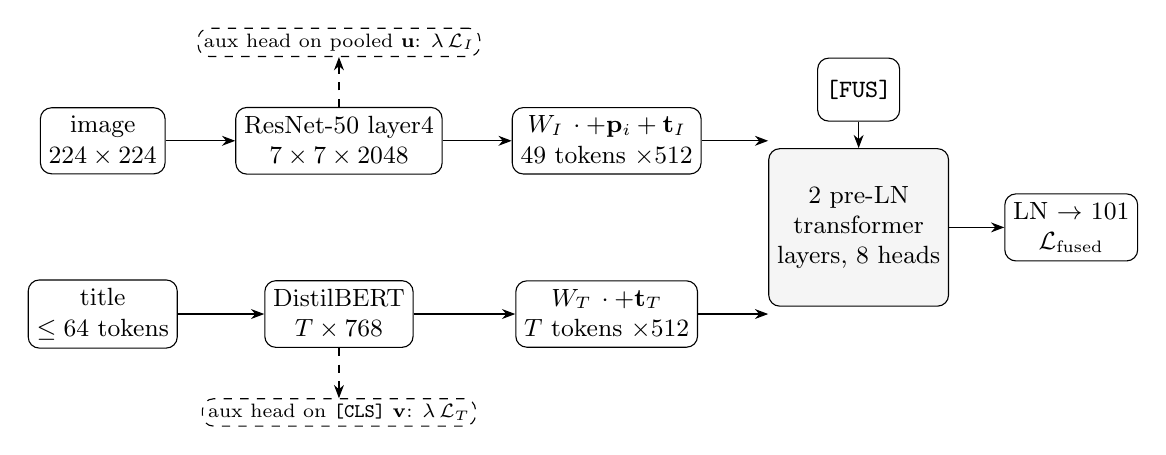
\begin{tikzpicture}[every node/.style={font=\small},
      box/.style={draw, rounded corners, align=center, minimum height=8mm, inner sep=3pt},
      aux/.style={draw, rounded corners, align=center, inner sep=2pt, font=\scriptsize, dashed},
      >={Stealth}]
    \node[box] (img) at (0,0) {image\\$224\times224$};
    \node[box] (rn)  at (3.0,0) {ResNet-50 layer4\\$7\times7\times2048$};
    \node[box] (pi)  at (6.4,0) {$W_I\,\cdot + \mathbf{p}_i + \mathbf{t}_I$\\49 tokens $\times 512$};
    \node[box] (txt) at (0,-2.2) {title\\$\le 64$ tokens};
    \node[box] (db)  at (3.0,-2.2) {DistilBERT\\$T\times768$};
    \node[box] (pt)  at (6.4,-2.2) {$W_T\,\cdot + \mathbf{t}_T$\\$T$ tokens $\times 512$};
    \node[box, fill=gray!8, minimum height=20mm] (tf) at (9.6,-1.1) {2 pre-LN\\transformer\\layers, 8 heads};
    \node[box] (fus) at (9.6,0.65) {\texttt{[FUS]}};
    \node[box] (head) at (12.3,-1.1) {LN $\to$ 101\\$\mathcal{L}_{\mathrm{fused}}$};
    \node[aux] (ai) at (3.0,1.25) {aux head on pooled $\mathbf{u}$: $\lambda\,\mathcal{L}_I$};
    \node[aux] (at) at (3.0,-3.45) {aux head on \texttt{[CLS]} $\mathbf{v}$: $\lambda\,\mathcal{L}_T$};
    \draw[->] (img) -- (rn); \draw[->] (txt) -- (db);
    \draw[->] (rn) -- (pi); \draw[->] (db) -- (pt);
    \draw[->] (pi.east) -- (tf.west |- pi.east); \draw[->] (pt.east) -- (tf.west |- pt.east);
    \draw[->] (fus) -- (tf); \draw[->] (tf) -- (head);
    \draw[->, dashed] (rn) -- (ai); \draw[->, dashed] (db) -- (at);
  \end{tikzpicture}
  \caption{F2. Image regions and title tokens attend to each other and to a learned \texttt{[FUS]} token, whose final
  state is classified. Dashed: auxiliary unimodal heads. During training, one modality of $15\%$ of the items is
  replaced by a learned \texttt{[MISSING]} token.}
  \label{fig:f2}
\end{figure}

\paragraph{Tokens.}
The image gives the ResNet-50 \texttt{layer4} map, i.e.\ $49$ region features $\mathbf{f}_i\in\R^{2048}$. The title
gives the DistilBERT hidden states $\mathbf{h}_j\in\R^{768}$, which already contain word positions. Both are projected
to $d=512$:
\begin{equation}
  \mathbf{z}^I_i = W_I\mathbf{f}_i + \mathbf{p}_i + \mathbf{t}_I, \qquad
  \mathbf{z}^T_j = W_T\mathbf{h}_j + \mathbf{t}_T, \qquad
  Z^{(0)} = [\,\mathbf{z}_{\mathrm{FUS}};\ \mathbf{z}^I_1,\dots,\mathbf{z}^I_{49};\ \mathbf{z}^T_1,\dots,\mathbf{z}^T_{T}\,],
\end{equation}
where $\mathbf{p}_i$ is a learned position embedding of the $7\times7$ grid, $\mathbf{t}_I,\mathbf{t}_T$ are learned
type embeddings and $\mathbf{z}_{\mathrm{FUS}}$ is a learned fusion token.

\paragraph{Fusion.}
Two pre-LN transformer layers~\cite{vaswani2017attention} ($8$ heads, FFN $2048$, dropout $0.1$) run self-attention
over the whole sequence. Padding tokens are masked. Every image region can therefore attend to every title word
and vice versa. The prediction is $f_{\mathrm{F2}} = W_o\LN(\mathbf{z}^{(2)}_{\mathrm{FUS}})$. A single fusion token
that gathers both modalities is close to the bottleneck tokens of Nagrani et al.~\cite{nagrani2021bottlenecks}.
Unlike F1, this design can weigh individual regions and words differently for every item. The \texttt{[FUS]}
attention also shows how much the model relies on each modality (\cref{sec:qualitative}).

\paragraph{Auxiliary unimodal losses.}
Two linear heads classify the pooled image feature $\mathbf{u}\in\R^{2048}$ and the text \texttt{[CLS]} state
$\mathbf{v}\in\R^{768}$:
\begin{equation}
  \label{eq:f2loss}
  \mathcal{L} = \CE\big(f_{\mathrm{F2}}, y\big) + \lambda\,\big[\CE(a_I(\mathbf{u}), y) + \CE(a_T(\mathbf{v}), y)\big],
  \qquad \lambda = 0.5 .
\end{equation}
Each encoder therefore has to stay discriminative on its own, so the image encoder keeps learning even when the
title already fits the training labels~\cite{wang2020makes}. The auxiliary heads are not used for the prediction.

\paragraph{Modality dropout and missing modalities.}
During training, each complete pair loses one modality with probability $p=0.15$ (image or title, $50/50$, never
both), in the spirit of ModDrop~\cite{neverova2016moddrop}. All tokens of the dropped modality are replaced by one
learned \texttt{[MISSING\_IMG]} or \texttt{[MISSING\_TXT]} token; the other positions of that modality are masked.
The fusion therefore learns to classify from one modality alone. At test time, a missing modality is handled in the
same way, with no special case. The auxiliary losses always see both encoders.

\paragraph{Training schedule.}
In epoch~1 both encoders are frozen and only the new layers learn ($5\cdot10^{-4}$). The randomly initialised fusion
layers then do not send noisy gradients into the pretrained encoders. From epoch~2, the whole model is fine-tuned
with the same learning rates as F1. The warm-up covers $15\%$ of the steps, so the encoders also start with a
warm-up after they are unfrozen. The model has $97.98$\,M parameters: $8.11$\,M new layers on top of the two
encoders. It needs $5.06$\,GMACs per item, against $4.73$ for F1.

\subsection{Ablations and Analyses}
\label{sec:ablations}

\begin{table}[H]
  \centering\small
  \caption{Controlled experiments. Each changes one factor of F2, or of the input, and keeps everything else, including
  the seeds and the split.}
  \label{tab:ablations}
  \begin{tabularx}{\linewidth}{@{}lYY@{}}
    \toprule
    ID & Change & Question \\
    \midrule
    E1 & $\lambda = 0$. The auxiliary heads are trained on detached features, so they still measure each encoder without changing it & Do the auxiliary losses keep the image branch alive? \\
    E2 & every class-name mention (the lexicon of Part~1) is replaced by \texttt{[MASK]} in the train, validation and test titles; UB, T0, F0, F1 and F2 are retrained & How much of the result depends on the label leaking into the title, and which fusion uses the image best when it does not? \\
    E4 & $p = 0$ (no modality dropout) & Does the modality dropout help with missing modalities, and does it cost anything on complete pairs? \\
    E-mod & at test time, the title (or the image) is removed from a random $0$, $25$, $50$, $75$ or $100\%$ of the complete pairs, without retraining & How fast does each model degrade when a modality goes missing? \\
    \bottomrule
  \end{tabularx}
\end{table}

\paragraph{Notes on the ablations.}
\begin{itemize}
  \item \textbf{E2 masking.} It changes $79.8\%$ of the training titles ($50{,}092$ of $62{,}771$). After masking, the
        lexicon finds no class name in any title. The mention subsets of \cref{sec:main} still use the original
        titles.
  \item \textbf{E-mod fallbacks.} For a removed modality, F1 zero-fills it and F2 uses its \texttt{[MISSING]} token.
        F0 falls back to the other unimodal model. UA and UB predict the most frequent training class.
\end{itemize}

\paragraph{Analyses.}
\begin{itemize}
  \item \textbf{Support/conflict groups} over three seeds. The groups come from the UA and UB runs of the same seed.
  \item \textbf{Temperature scaling}~\cite{guo2017calibration}: one temperature per run, fitted on validation.
  \item \textbf{Qualitative examples} for each group:
        \begin{itemize}
          \item a Grad-CAM map~\cite{selvaraju2017gradcam} of F2's image encoder for the predicted class;
          \item the \texttt{[FUS]} attention of the last fusion layer, averaged over heads.
        \end{itemize}
  \item \textbf{Error taxonomy} from a manual review of $100$ conflict items, 50 Conflict-I and 50 Conflict-T,
        drawn at random from seed 42. Each reviewer chose the main reason why the failing unimodal model is wrong:
        \begin{itemize}
          \item image unrelated or visually similar (for the image model);
          \item title generic or title naming another dish (for the text model);
          \item wrong label or other (for both).
        \end{itemize}
        Phan Bá Thanh reviewed items 1--50 and Trần Công Hoàng Phước items 51--100. Hard cases were discussed
        together.
\end{itemize}

\subsection{Pretraining and Fine-Tuning}
\label{sec:training}

Both encoders start from public pretrained weights and are fully fine-tuned with discriminative learning rates.
\Cref{tab:setup} lists the setup; only the noted values differ between models.

\begin{table}[H]
  \centering\small
  \caption{Training setup.}
  \label{tab:setup}
  \begin{tabularx}{\linewidth}{@{}lY@{}}
    \toprule
    Image transforms & train: \texttt{RandomResizedCrop(224, scale 0.35--1)}, horizontal flip, colour jitter $0.1$; evaluation: \texttt{Resize(256)} + \texttt{CenterCrop(224)} \\
    Optimiser & AdamW~\cite{loshchilov2019adamw}. Learning rates: image encoder $10^{-4}$, text encoder $3\cdot10^{-5}$, new layers $10^{-3}$ (UA, UB) or $5\cdot10^{-4}$ (F1, F2). Weight decay $0.05$ (image encoder and heads), $0.01$ (text encoder); none on biases and normalisation parameters \\
    Schedule & linear warm-up over $5\%$ of the steps, then cosine decay to $1\%$ \\
    Epochs, batch & UA and F1: 10 epochs; UB: 5 epochs; batch size 64; bf16 autocast; gradient clipping at $1.0$ \\
    F2 and its ablations & as F1, plus: epoch 1 with frozen encoders, warm-up over $15\%$ of the steps, head learning rate $5\cdot10^{-4}$ \\
    Checkpoint & the epoch with the best validation macro-F1 on complete pairs; early stopping after 3 epochs without improvement \\
    Seeds & split seed $42$ (fixed); training seeds $42$, $123$, $2026$ \\
    \bottomrule
  \end{tabularx}
\end{table}

\subsection{Evaluation Protocol}
\label{sec:protocol}

\paragraph{Metrics.}
\begin{itemize}
  \item Macro-F1 (primary), top-1 and top-5 accuracy.
  \item Expected calibration error with $15$ equal-width bins~\cite{guo2017calibration},
        $\mathrm{ECE}=\sum_b \frac{|B_b|}{N}\,|\mathrm{acc}(B_b)-\mathrm{conf}(B_b)|$.
  \item Per-class F1 and the confusion matrix.
  \item Compute cost: parameters, training time, throughput at batch 128 and latency at batch 1.
\end{itemize}

\paragraph{Decision rule.}
The rule is the same as in A1 and A2 and was registered in the proposal. Model~A is declared better than model~B
only if both conditions hold:
\begin{enumerate}
  \item the difference in mean test macro-F1 over the three seeds exceeds the larger of the two seed standard deviations;
  \item a McNemar test~\cite{mcnemar1947} on the seed-42 predictions rejects equal error rates at $p<0.05$.
\end{enumerate}

\paragraph{Test views.}
Every model is evaluated on:
\begin{itemize}
  \item the complete test pairs ($22{,}594$);
  \item the dedup subset;
  \item the title-unseen subset;
  \item titles that do or do not mention the true class;
  \item the natural missing-text set ($121$ items).
\end{itemize}
The fusion models are also tested with each modality removed.

\subsection{Hardware and Software}
\label{sec:hardware}

The Kaggle GPU quota ran out during M2, so all training runs (M2 and M3) used a lab workstation:
\begin{itemize}
  \item \textbf{GPU:} NVIDIA RTX A6000 (48\,GB), shared with other users' inference servers.
  \item \textbf{Machine:} 64 CPU cores, Ubuntu 24.04.
  \item \textbf{Software:} Python 3.13.13, PyTorch 2.12.0+cu130, torchvision 0.27.0, Transformers 5.23.0, CUDA 13.0.
\end{itemize}
The runner (\texttt{scripts/remote/}) runs inside \texttt{tmux}. It picks the GPU with the most free memory
(32\,GB free at the start), logs the GPU usage every five minutes, and resumes from the last checkpoint after a
crash; no crash occurred in either milestone. Data preparation ran on a Kaggle CPU notebook with 4 vCPU
(26 minutes). The M3 runs used the same machine, software and $16$ data-loading workers. T0 and the analyses ran
on the CPU of the same machine.


\part*{Part 3: Implementation Results}
\addcontentsline{toc}{part}{Part 3: Implementation Results}
% =====================================================================
%  Part 3: Implementation results
% =====================================================================
\section{Implementation Results}
\label{sec:results}

Unless stated otherwise, the numbers are test results on the $22{,}594$ complete pairs. They are given as
mean~$\pm$~sample standard deviation over the training seeds $42$, $123$ and $2026$. K0 and T0 are deterministic,
so each has a single value.

\subsection{Training Behaviour}
\label{sec:curves}

\begin{figure}[H]
  \centering
  \begin{subfigure}{0.49\linewidth}
    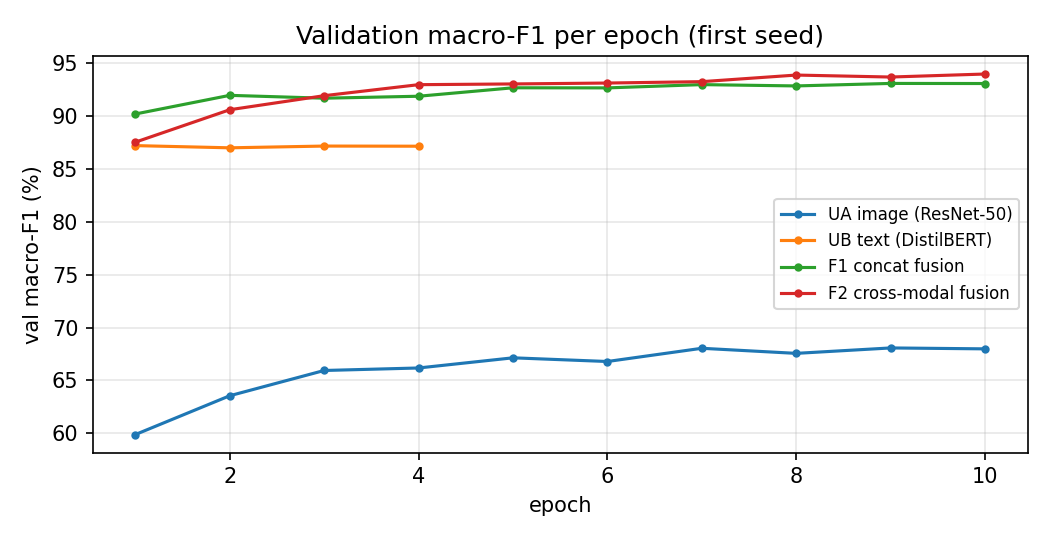
\includegraphics[width=\linewidth]{val_curves.png}
    \caption{Validation macro-F1 per epoch (one seed).}
  \end{subfigure}\hfill
  \begin{subfigure}{0.49\linewidth}
    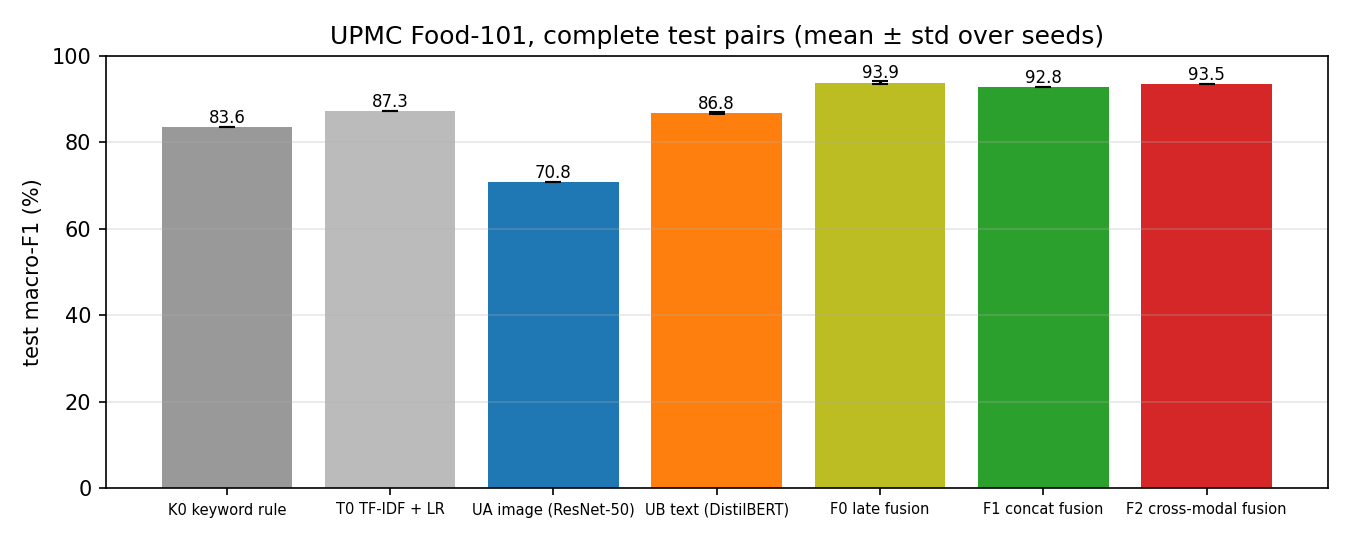
\includegraphics[width=\linewidth]{macro_f1.png}
    \caption{Test macro-F1, mean $\pm$ std.}
  \end{subfigure}
  \caption{Training behaviour and the main result.}
  \label{fig:curves}
\end{figure}

\begin{itemize}
  \item \textbf{UA} improves slowly. Its validation macro-F1 stays around $68\%$; the best epoch is $9$ of $10$.
  \item \textbf{UB} converges after one epoch, at $87\%$ validation macro-F1.
  \item \textbf{F1} starts at $90\%$ after one epoch and fits the training set to $99.7\%$ accuracy.
  \item \textbf{F2}:
        \begin{itemize}
          \item reaches $87.5\%$ after the frozen-encoder epoch, which trains only the $8$\,M new parameters;
          \item passes F1 from epoch~3 and ends at $93.9\%$, with the best epoch between $8$ and $10$;
          \item fits the training set less tightly than F1 ($97.2\%$ against $99.7\%$ accuracy), because the
                auxiliary losses and the modality dropout make the training task harder;
          \item has an auxiliary image head that reaches $68\%$ validation accuracy, as high as the standalone
                image model.
        \end{itemize}
\end{itemize}

\subsection{Unimodal versus Multimodal}
\label{sec:main}

\begin{table}[H]
  \centering\small
  \caption{Main comparison on the complete test pairs. ``Dedup'' removes test items whose image is linked to a
  train image. ``Title unseen'' keeps only the $13{,}701$ test items whose title never occurs in train or validation.}
  \label{tab:main}
  \resizebox{\linewidth}{!}{%
  \begin{tabular}{@{}lcccccc@{}}
    \toprule
    Model & Accuracy & Macro-F1 & Top-5 & ECE & Macro-F1 dedup & Macro-F1 title unseen \\
    \midrule
    K0 keyword rule & $76.95$ & $83.56$ & $77.41$ & $2.97$ & $83.81$ & $82.89$ \\
    T0 TF-IDF + LR  & $87.12$ & $87.26$ & $91.23$ & $2.71$ & $87.36$ & $82.57$ \\
    UA image        & $70.73\pm0.09$ & $70.80\pm0.06$ & $86.51\pm0.16$ & $10.75\pm0.19$ & $67.72\pm0.03$ & $70.59\pm0.12$ \\
    UB text         & $86.42\pm0.91$ & $86.80\pm0.25$ & $90.71\pm0.69$ & $2.84\pm1.46$ & $86.96\pm0.07$ & $82.57\pm0.44$ \\
    \midrule
    F0 late fusion  & $\mathbf{93.93\pm0.23}$ & $\mathbf{93.86\pm0.24}$ & $\mathbf{97.71\pm0.07}$ & $15.98\pm0.78$ & $\mathbf{93.71\pm0.27}$ & $\mathbf{92.03\pm0.32}$ \\
    F1 concat fusion & $92.85\pm0.06$ & $92.80\pm0.06$ & $97.15\pm0.04$ & $4.69\pm0.02$ & $92.80\pm0.07$ & $90.28\pm0.03$ \\
    F2 cross-modal fusion & $93.58\pm0.07$ & $93.53\pm0.07$ & $97.69\pm0.04$ & $\mathbf{2.88\pm0.09}$ & $93.49\pm0.06$ & $91.05\pm0.14$ \\
    \bottomrule
  \end{tabular}}
\end{table}

\begin{table}[H]
  \centering\small
  \caption{Decision rule. $b$ = items that only A classifies correctly, $c$ = items that only B classifies
  correctly (seed 42). A verdict needs both $|\Delta| >$ the larger std and $p<0.05$.}
  \label{tab:decision}
  \begin{tabular}{@{}lrrrrl@{}}
    \toprule
    A vs B & $\Delta$ macro-F1 (pp) & Larger std & $b$ / $c$ & McNemar $p$ & Verdict \\
    \midrule
    UB vs K0 & $+3.24$  & $0.25$ & $2{,}031$ / $128$     & $<10^{-300}$ & UB better \\
    UB vs T0 & $-0.46$  & $0.25$ & $260$ / $655$         & $9\cdot10^{-39}$ & T0 better \\
    UB vs UA & $+16.00$ & $0.25$ & $5{,}503$ / $2{,}219$ & $2\cdot10^{-305}$ & UB better \\
    F0 vs UB & $+7.06$  & $0.25$ & $2{,}068$ / $178$     & $<10^{-300}$ & F0 better \\
    F1 vs UB & $+6.00$  & $0.25$ & $1{,}868$ / $161$     & $<10^{-300}$ & F1 better \\
    F2 vs UB & $+6.73$  & $0.25$ & $2{,}036$ / $168$     & $<10^{-300}$ & F2 better \\
    F1 vs F0 & $-1.06$  & $0.24$ & $426$ / $609$         & $1.5\cdot10^{-8}$ & F0 better \\
    \textbf{F2 vs F1} & $+0.73$ & $0.07$ & $439$ / $278$ & $2.3\cdot10^{-9}$ & \textbf{F2 better} \\
    \textbf{F2 vs F0} & $-0.33$ & $0.24$ & $465$ / $487$ & $0.50$ & \textbf{no decision} \\
    \bottomrule
  \end{tabular}
\end{table}

\begin{enumerate}
  \item \textbf{Text dominates the unimodal results.}
        \begin{itemize}
          \item UB is $16$\,pp above UA, as the proposal hypothesised (E0).
          \item The simple TF-IDF model T0 is even slightly better than UB on the full test set ($+0.46$\,pp,
                significant).
          \item On titles that also occur in training, T0 is more accurate than UB ($93.2$ against $91.7\%$);
                on unseen titles the two are equal ($82.6\%$ macro-F1). The TF-IDF model memorises repeated
                titles a little better. Fine-tuning DistilBERT does not pay off on short titles that mostly name
                the dish.
        \end{itemize}
  \item \textbf{Every fusion clearly beats every unimodal model}, by $6$--$7$\,pp. This holds on the full test set,
        on the dedup subset and on the title-unseen subset.
  \item \textbf{F2 improves over the trained baseline F1} by $0.73$\,pp. The gain is significant, far above the
        seed spread ($0.07$), and also holds on the title-unseen subset ($+0.77$\,pp).
  \item \textbf{F2 does not beat the late fusion F0.} The difference ($-0.33$\,pp) is smaller than F0's seed spread,
        and McNemar finds no difference ($465$ against $487$ discordant items). On complete pairs with informative
        titles, a learned fusion has little to add to averaging two strong unimodal predictions.
        \Cref{sec:e2} shows that this changes when the title carries less direct information.
\end{enumerate}

\subsection{Ablations}
\label{sec:ablation-results}

\subsubsection{E1: auxiliary unimodal losses}

\begin{table}[H]
  \centering\small
  \caption{E1. ``Image head'' and ``text head'' are the accuracies of the auxiliary heads. Without the auxiliary
  losses they are linear probes on the detached features.}
  \label{tab:e1}
  \resizebox{\linewidth}{!}{%
  \begin{tabular}{@{}lcccccc@{}}
    \toprule
    Model & Macro-F1 & Image head & Text head & Acc.\ title removed & Acc.\ image removed & Missing-text set \\
    \midrule
    F2 ($\lambda=0.5$)     & $\mathbf{93.53\pm0.07}$ & $\mathbf{69.7\pm0.4}$ & $\mathbf{87.1\pm0.0}$ & $\mathbf{65.3\pm0.9}$ & $86.7\pm0.2$ & $61.4\pm0.5$ \\
    E1 ($\lambda=0$)       & $93.07\pm0.08$ & $62.3\pm0.1$ & $76.8\pm1.7$ & $58.6\pm0.8$ & $86.3\pm0.1$ & $53.7\pm3.0$ \\
    \bottomrule
  \end{tabular}}
\end{table}

\begin{itemize}
  \item \textbf{Verdict.} The auxiliary losses help: $+0.46$\,pp macro-F1, above the larger std ($0.08$), with
        McNemar $p=3\cdot10^{-7}$.
  \item \textbf{They keep the encoders discriminative.} A linear probe on the image features of E1 reaches only
        $62.3\%$, while the image head of F2 reaches $69.7\%$, close to the standalone UA ($70.7\%$). Without the
        auxiliary losses, joint training lets the image encoder drift away from features that separate the
        classes on their own. This is the ``modality laziness'' seen in F1 in M2. The text features are affected
        even more ($76.8$ against $87.1\%$).
  \item \textbf{Most of the benefit shows when the title is missing}: $+6.7$\,pp with the title removed and $+7.7$\,pp
        on the natural missing-text set. With the image removed, the gain is only $+0.4$\,pp, so the losses
        mainly protect the weaker modality.
\end{itemize}

\subsubsection{E4: modality dropout}

\begin{table}[H]
  \centering\small
  \caption{E4. The natural missing-text set has $121$ items; ``[MISSING]'' feeds the learned missing token instead of the uninformative title.}
  \label{tab:e4}
  \resizebox{\linewidth}{!}{%
  \begin{tabular}{@{}lccccc@{}}
    \toprule
    Model & Macro-F1 & Acc.\ title removed & Acc.\ image removed & Missing-text, as is & Missing-text, [MISSING] \\
    \midrule
    F2 ($p=0.15$) & $93.53\pm0.07$ & $\mathbf{65.3\pm0.9}$ & $86.7\pm0.2$ & $61.4\pm0.5$ & $60.6\pm2.4$ \\
    E4 ($p=0$)    & $93.45\pm0.06$ & $60.6\pm0.4$ & $86.5\pm0.0$ & $58.1\pm1.9$ & $57.9\pm1.4$ \\
    \bottomrule
  \end{tabular}}
\end{table}

\begin{itemize}
  \item \textbf{Verdict on complete pairs: no decision.} The difference is $+0.08$\,pp (McNemar $p=0.54$). The
        modality dropout costs nothing on complete pairs.
  \item \textbf{It helps when the title is missing}: $+4.7$\,pp accuracy with the title removed. It barely matters
        when the image is missing, because the title alone is already almost as good as the full input.
  \item \textbf{Even with both mechanisms, F2 stays below UA without the title} ($65.3$ against $70.7\%$). F0 falls
        back to UA by construction, so it is the most robust model for a missing title (\cref{sec:emod}).
\end{itemize}

\subsubsection{E2: class names masked}
\label{sec:e2}

\begin{table}[H]
  \centering\small
  \caption{E2. Every model is retrained and tested on titles in which every class-name mention is replaced by
  \texttt{[MASK]}. ``Gain over UB'' is the macro-F1 gain of the fusion over the text model of the same seed.}
  \label{tab:e2}
  \resizebox{\linewidth}{!}{%
  \begin{tabular}{@{}lccccc@{}}
    \toprule
    Model & Macro-F1 as is & Macro-F1 masked & $\Delta$ (pp) & Gain over UB, as is & Gain over UB, masked \\
    \midrule
    T0 TF-IDF  & $87.26$ & $47.79$ & $-39.5$ & -- & -- \\
    UB text    & $86.80\pm0.25$ & $43.70\pm0.16$ & $-43.1$ & -- & -- \\
    F0 late    & $\mathbf{93.86\pm0.24}$ & $78.85\pm0.17$ & $-15.0$ & $7.1$ & $35.2$ \\
    F1 concat  & $92.80\pm0.06$ & $80.43\pm0.14$ & $-12.4$ & $6.0$ & $36.7$ \\
    F2 cross-modal & $93.53\pm0.07$ & $\mathbf{81.31\pm0.02}$ & $-12.2$ & $6.7$ & $\mathbf{37.6}$ \\
    \bottomrule
  \end{tabular}}
\end{table}

\begin{itemize}
  \item \textbf{Half of the text signal is the class name.}
        \begin{itemize}
          \item Masking halves the text-only models: UB falls from $86.8$ to $43.7\%$, T0 from $87.3$ to $47.8\%$.
          \item On titles that never named the class, UB scores $39.2\%$ without masking and $39.7\%$ with it, so
                the masking removes the name and nothing else.
          \item What remains in a masked title (ingredients, cooking words, site names, repeated titles) is still
                worth $44\%$, far above chance ($1\%$) but below the image ($70.8\%$). The masked text model is
                $67\%$ accurate on titles seen in train and $28\%$ on unseen ones, so a large part of the
                remainder is memorised page titles.
        \end{itemize}
  \item \textbf{Fusion is much more valuable on masked titles.} The gain over the text model grows from about
        $7$\,pp to $35$--$38$\,pp. All three fusions are also $8$--$11$\,pp above the image model, so the weak
        title still adds information.
  \item \textbf{F2 is the best fusion on masked titles.} It beats F1 by $0.88$\,pp ($p=2\cdot10^{-4}$) and F0 by
        $2.46$\,pp ($p=2\cdot10^{-28}$), with the smallest seed spread ($0.02$). When neither modality is decisive,
        token-level cross-attention combines the partial evidence better than averaging two probability vectors.
        This reverses the F0--F1 ranking of the unmasked titles.
\end{itemize}

\subsection{Modality Removal (E-mod) and Missing Modality}
\label{sec:emod}

\begin{figure}[H]
  \centering
  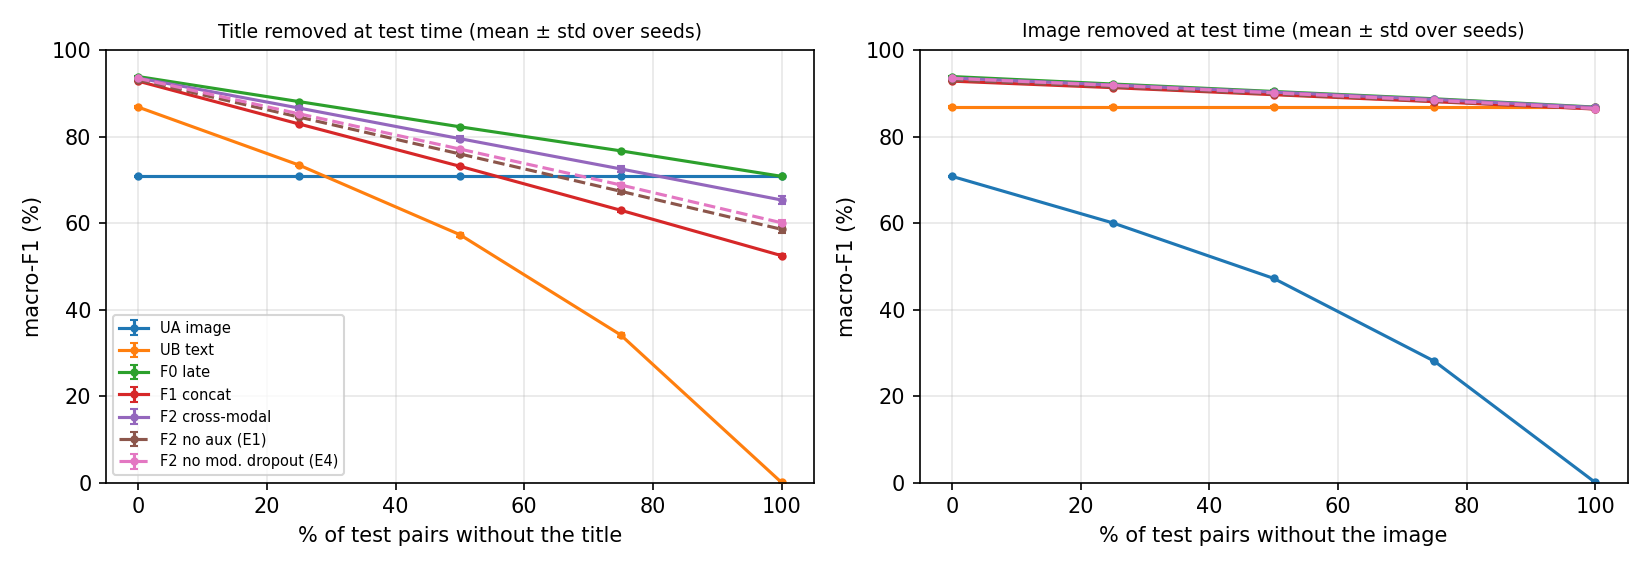
\includegraphics[width=\linewidth]{removal_curves.png}
  \caption{Macro-F1 when the title (left) or the image (right) is removed from a random fraction of the complete
  test pairs, without retraining. Removed items use each model's fallback (\cref{sec:ablations}).}
  \label{fig:removal}
\end{figure}

\begin{itemize}
  \item \textbf{Linear curves.} The removed items are drawn at random, so each curve is a linear mix of the
        full-input and the single-modality accuracy. The end points carry all the information; the slope shows how
        much each model depends on a modality.
  \item \textbf{Removing the image costs every fusion about $7$\,pp.} All fusions end at the text model's level
        ($86.3$--$86.8\%$).
  \item \textbf{Removing the title separates the models}, as shown by macro-F1 with $100\%$ of the titles removed:
        \begin{itemize}
          \item F0: $70.8\%$, because it falls back to UA;
          \item F2: $65.3\%$;
          \item F2 without modality dropout (E4): $60.1\%$;
          \item F2 without auxiliary losses (E1): $58.5\%$;
          \item F1: $52.5\%$.
        \end{itemize}
        F2's two mechanisms close more than half of F1's gap to the image model, but not all of it.
  \item \textbf{Natural missing-text set} ($121$ items with an invalid title), accuracy:
        \begin{itemize}
          \item UA: $65.6\%$; UB: $6.3\%$;
          \item F0: $68.9\%$ with the title as is;
          \item F2: $61.4\%$ with the title as is, $60.6\%$ with its \texttt{[MISSING]} token;
          \item F1: $51.8\%$. This value comes from the M2 evaluation, which zero-filled the text in both
                variants.
        \end{itemize}
\end{itemize}

\subsection{Support and Conflict Analysis (three seeds)}
\label{sec:support}

\begin{table}[H]
  \centering\small
  \caption{Fusion accuracy per group, mean over seeds. The groups come from UA and UB of the same seed.
  ``Follows image'' = share of items where the fused prediction equals UA's.}
  \label{tab:support}
  \resizebox{\linewidth}{!}{%
  \begin{tabular}{@{}lrrrrrrrr@{}}
    \toprule
    Group & Items & Share & F0 & F1 & F2 & E1 & E4 & F2 follows image \\
    \midrule
    Support (both right)          & $13{,}938$ & $61.7\%$ & $100.0$ & $99.8$ & $99.8$ & $99.8$ & $99.8$ & $99.8\%$ \\
    Conflict-I (only image right) & $2{,}043$  & $9.0\%$  & $\mathbf{90.6\pm4.5}$ & $69.0\pm2.7$ & $75.3\pm2.0$ & $70.9\pm1.3$ & $74.7\pm1.6$ & $75.3\%$ \\
    Conflict-T (only text right)  & $5{,}588$  & $24.7\%$ & $97.1\pm0.9$ & $97.7\pm0.1$ & $97.7\pm0.2$ & $\mathbf{97.9\pm0.2}$ & $97.8\pm0.2$ & $1.2\%$ \\
    Both wrong, same prediction   & $150$      & $0.7\%$  & $0.0$ & $10.7$ & $10.6$ & $10.7$ & $10.0$ & $84.3\%$ \\
    Both wrong, different         & $875$      & $3.9\%$  & $0.7$ & $21.3$ & $\mathbf{24.0}$ & $22.6$ & $23.2$ & $18.9\%$ \\
    \bottomrule
  \end{tabular}}
\end{table}

\begin{figure}[H]
  \centering
  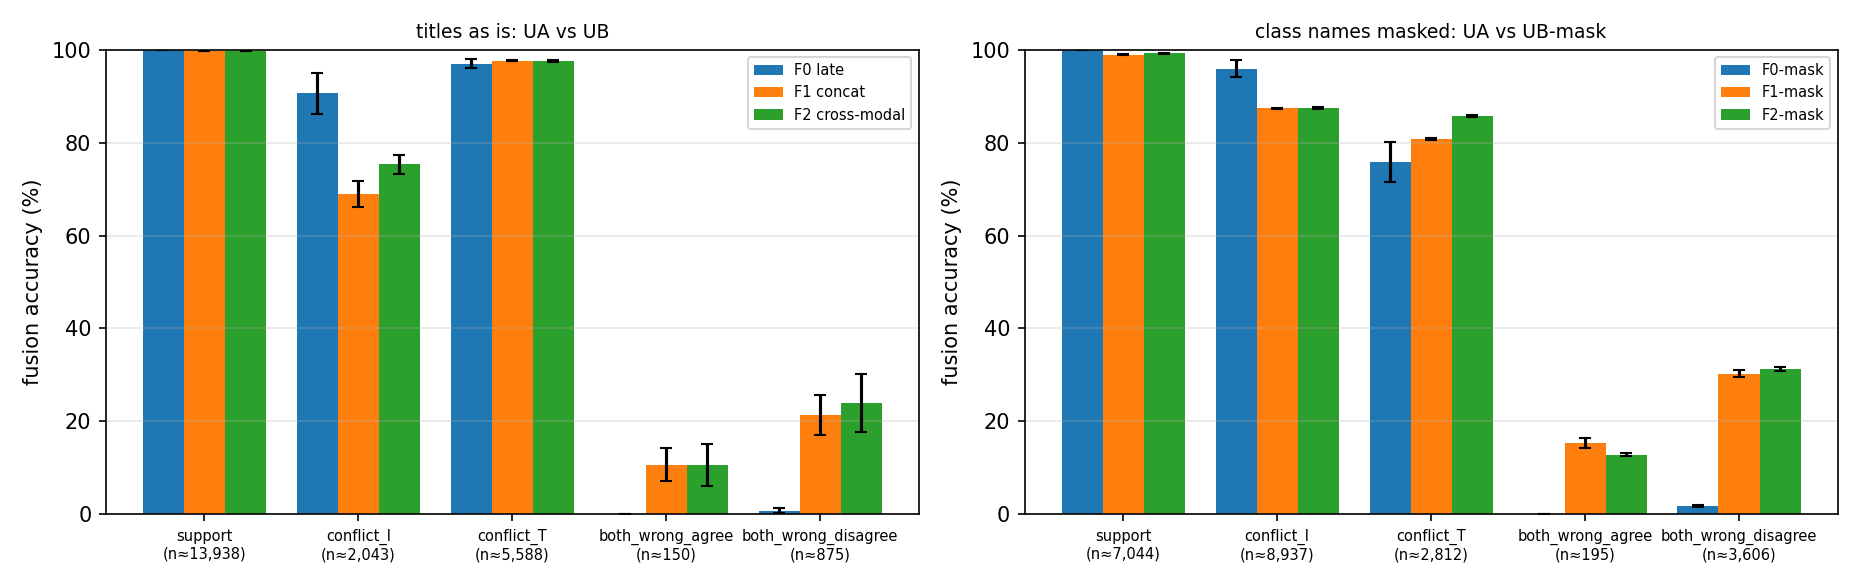
\includegraphics[width=\linewidth]{support_conflict_seeds.png}
  \caption{Fusion accuracy per group over three seeds, with titles as is (left) and with class names masked (right).}
  \label{fig:support}
\end{figure}

\begin{itemize}
  \item \textbf{Stable over seeds.} The M2 conclusions (seed 42 only) hold over three seeds:
        \begin{itemize}
          \item support items are solved by every model;
          \item the fusion gain comes from the conflict groups;
          \item a misleading title (Conflict-I) is the weak spot of the trained fusions.
        \end{itemize}
  \item \textbf{Conflict-I.} F2 recovers $75.3\%$ of these items, against $69.0\%$ for F1. This is $+6.3$\,pp, and
        E1 shows that the auxiliary losses account for most of it ($70.9\%$ without them). F0 still recovers the
        most ($90.6\%$). Its averaging lets a confident image prediction outvote an uncertain title, while F2 still
        follows the title in a quarter of these items.
  \item \textbf{Both wrong.} The trained fusions are the only models that solve some items on which both unimodal
        models fail. F2 solves $24\%$ of the items where UA and UB disagree. A late fusion can only choose between
        the two unimodal predictions, so it cannot do this.
  \item \textbf{With masked titles (right panel), the balance shifts.} Conflict-I becomes the largest group
        ($40\%$). F2-mask is the best model on Conflict-T ($85.7\%$ against $75.9\%$ for F0-mask) and on the
        items where both unimodal models are wrong and disagree ($31.2\%$). This is where its overall advantage on masked titles comes from.
\end{itemize}

\subsection{Qualitative Analysis: Grad-CAM and \texttt{[FUS]} Attention}
\label{sec:qualitative}

\begin{figure}[H]
  \centering
  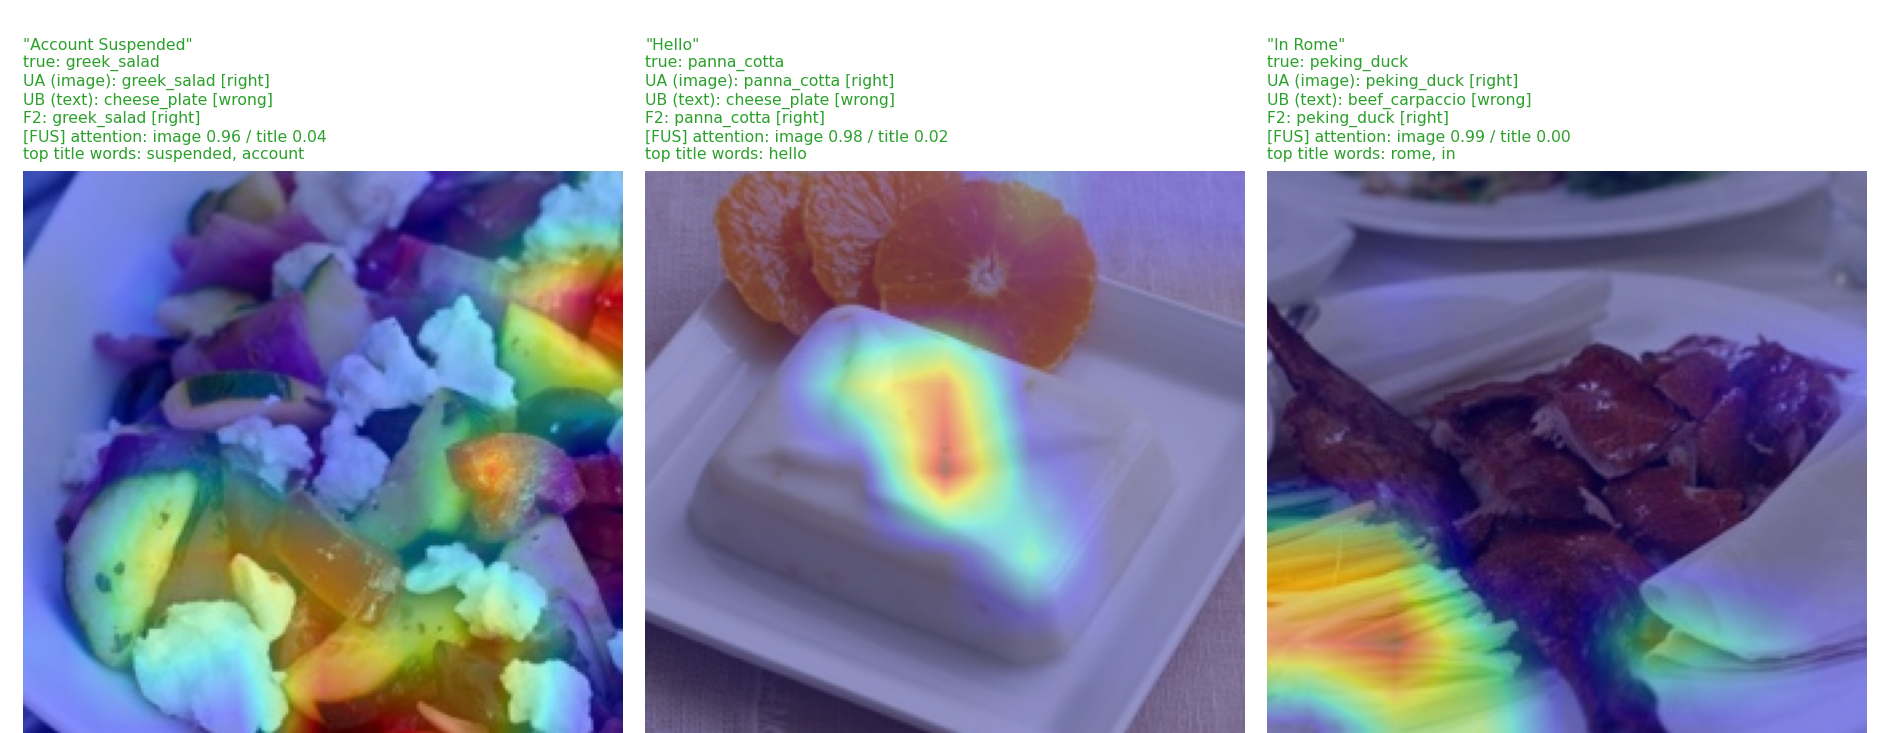
\includegraphics[width=\linewidth]{qual_conflict_I.png}
  \caption{Conflict-I examples (seed 42): the image model is right and the text model is wrong. Grad-CAM of F2's
  image encoder for F2's predicted class; title in green if F2 is right.}
  \label{fig:qual-i}
\end{figure}

\begin{figure}[H]
  \centering
  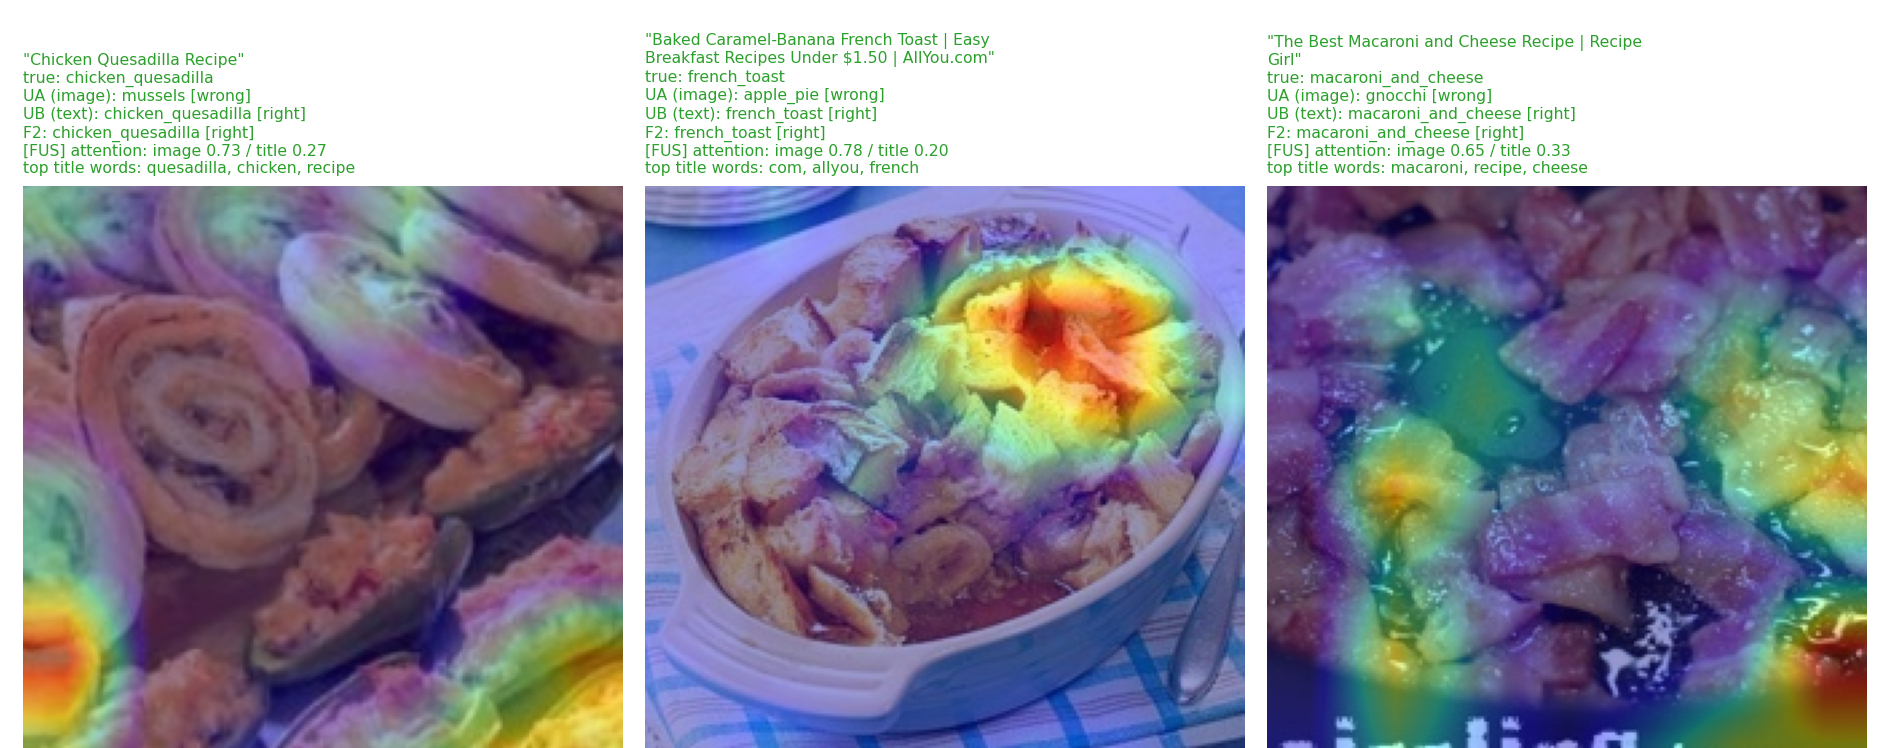
\includegraphics[width=\linewidth]{qual_conflict_T.png}
  \caption{Conflict-T examples (seed 42): the text model is right and the image model is wrong.}
  \label{fig:qual-t}
\end{figure}

\begin{table}[H]
  \centering\small
  \caption{Mean share of the \texttt{[FUS]} attention on the image tokens (last fusion layer, seed 42). The rest goes
  to the title tokens and to \texttt{[FUS]} itself.}
  \label{tab:attention}
  \begin{tabular}{@{}lccccc@{}}
    \toprule
    Model & All & Support & Conflict-I & Conflict-T & Both wrong \\
    \midrule
    F2       & $0.805$ & $0.792$ & $\mathbf{0.909}$ & $0.778$ & $0.891$ \\
    E1 (no aux.) & $0.756$ & $0.745$ & $0.873$ & $0.720$ & $0.847$ \\
    E4 (no mod.\ dropout) & $0.883$ & $0.883$ & $0.930$ & $0.858$ & $0.917$ \\
    F2-mask  & $0.922$ & $0.928$ & $0.927$ & $0.907$ & $0.912$ \\
    \bottomrule
  \end{tabular}
\end{table}

\begin{itemize}
  \item \textbf{F2 shifts its attention item by item.} On Conflict-I items, whose titles are uninformative, $91\%$
        of the \texttt{[FUS]} attention goes to the image. On Conflict-T items it is $78\%$. In
        \cref{fig:qual-i}, titles such as ``Account Suspended'', ``Hello'' or ``In Rome'' get $0$--$4\%$ of the
        attention, and F2 classifies from the image. In \cref{fig:qual-t}, the title words that name the dish
        (``quesadilla'', ``macaroni'', ``cheese'') receive the most attention.
  \item \textbf{The shares should be compared between groups, not read as absolute values.} The image has $49$
        tokens against about $15$ for a title, so a uniform attention would already give about $0.75$ to the
        image. E1 attends less to the image ($0.756$), which fits its weaker image branch. F2-mask attends more
        ($0.922$), which fits a less informative title.
  \item \textbf{Grad-CAM} usually highlights the food rather than the plate or the background. Two kinds of failure
        recur:
        \begin{itemize}
          \item the map spreads over a mix of dishes, for example the starter platter labelled
                \cls{chicken\_quesadilla} in \cref{fig:qual-t};
          \item the map lands on text overlaid on the image (``sizzling bacon'').
        \end{itemize}
        Both are cases where the image alone is misleading and the title has to decide.
\end{itemize}

\subsection{Error Taxonomy of the Conflict Cases}
\label{sec:taxonomy}

\begin{table}[H]
  \centering\small
  \caption{Main cause of the failing unimodal model in $100$ random conflict items (seed 42), with Wilson 95\%
  intervals~\cite{wilson1927}. The last three columns give the accuracy of the fusion models on the same items.}
  \label{tab:taxonomy}
  \resizebox{\linewidth}{!}{%
  \begin{tabular}{@{}llrrrrr@{}}
    \toprule
    Group (failing model) & Cause & Items & Share (95\% CI) & F0 & F1 & F2 \\
    \midrule
    Conflict-I (text wrong)  & title generic (no dish information)   & $42$ & $84\%$ ($71$--$92$) & $100$ & $74$ & $93$ \\
                             & title names another dish             & $8$  & $16\%$ ($8$--$29$)  & $50$ & $38$ & $50$ \\
    \midrule
    Conflict-T (image wrong) & visually similar to another dish     & $34$ & $68\%$ ($54$--$79$) & $94$ & $94$ & $100$ \\
                             & image unrelated (no dish, collage, \dots) & $13$ & $26\%$ ($16$--$40$) & $100$ & $100$ & $100$ \\
                             & wrong label                          & $2$  & $4\%$ ($1$--$13$)   & $100$ & $100$ & $100$ \\
                             & other                                & $1$  & $2\%$ ($0$--$10$)   & $100$ & $100$ & $100$ \\
    \bottomrule
  \end{tabular}}
\end{table}

\begin{itemize}
  \item \textbf{The text model fails mostly on generic titles}, such as a site name, ``Hello'' or a drinks brand,
        not on wrong ones. F0 and F2 fix almost all of these items; F1 fixes only three quarters.
  \item \textbf{The hard case is a title that names another dish}, for example ``French Bread Pizza'' for a
        \cls{pizza} image, which UB reads as \cls{garlic\_bread}. Every fusion solves only about half of these
        items, because the title actively points to a wrong class instead of carrying no information.
  \item \textbf{The image model fails mostly on dishes that look alike} or on unusual plating, such as a beef
        tartare tower topped with caviar that it reads as cupcakes. Here F2 is the only model that solves every
        reviewed item.
  \item \textbf{Wrong labels are rare} ($2$ of $100$), in line with the $0.5\%$ of the M2 pair audit.
  \item \textbf{Repeated titles.} In $28\%$ of the reviewed items, the title also occurs in train or
        validation. Some correct text predictions are memorised: the title ``- quoteko.com'' occurs $80$ times in
        train and validation, $77$ of them as \cls{breakfast\_burrito}, so UB predicts that class with $98\%$
        confidence for an image of baked oatmeal. Other correct text predictions are lucky guesses with a
        confidence of a few percent.
  \item \textbf{Limitations.} The sample is small: the ``another dish'' group has $8$ items. Each item was labelled
        by one reviewer, so there is no inter-rater agreement.
\end{itemize}

\subsection{Leakage Checks}
\label{sec:leakage}

\begin{table}[H]
  \centering\small
  \caption{Accuracy on test titles that do or do not occur in train/validation, and macro-F1 on unseen titles.}
  \label{tab:leakage}
  \begin{tabular}{@{}lrrr@{}}
    \toprule
    Model & Acc.\ title seen ($8{,}893$) & Acc.\ title unseen ($13{,}701$) & Macro-F1 unseen \\
    \midrule
    UA image  & $70.18$ & $71.09$ & $70.59$ \\
    UB text   & $91.71$ & $82.99$ & $82.57$ \\
    T0 TF-IDF & $93.24$ & $83.14$ & $82.57$ \\
    F0 late   & $95.88$ & $92.67$ & $\mathbf{92.03}$ \\
    F1 concat & $95.76$ & $90.96$ & $90.28$ \\
    F2 cross-modal & $96.44$ & $91.73$ & $91.05$ \\
    \bottomrule
  \end{tabular}
\end{table}

\begin{itemize}
  \item \textbf{Repeated titles inflate every text-using model by $3$--$10$\,pp.} The image model, which never sees
        the title, is a control: it is as accurate on both subsets.
  \item \textbf{The ranking and every decision of \cref{tab:decision} hold on the title-unseen subset.} F2 is
        $0.77$\,pp above F1 and $1.0$\,pp below F0 there.
  \item \textbf{Image duplicates} inflate only the image model ($-3.1$\,pp on the dedup subset). Every fusion
        loses at most $0.2$\,pp there.
\end{itemize}

\subsection{Calibration}
\label{sec:calibration}

\begin{table}[H]
  \centering\small
  \caption{Test ECE (\%) before and after temperature scaling; $T$ is fitted on validation.}
  \label{tab:calibration}
  \resizebox{\linewidth}{!}{%
  \begin{tabular}{@{}lrrr@{\hspace{2em}}lrrr@{}}
    \toprule
    Model & $T$ & Before & After & Model & $T$ & Before & After \\
    \midrule
    UA & $1.62$ & $10.75$ & $4.22$ & F2 & $1.40$ & $\mathbf{2.88}$ & $\mathbf{0.45}$ \\
    UB & $1.30$ & $2.84$ & $1.01$  & E1 & $1.39$ & $3.02$ & $0.59$ \\
    F0 & $0.61$ & $15.98$ & $6.46$ & E4 & $1.59$ & $3.57$ & $0.56$ \\
    F1 & $1.91$ & $4.69$ & $0.90$  & F2-mask & $1.50$ & $8.43$ & $0.83$ \\
    \bottomrule
  \end{tabular}}
\end{table}

\begin{itemize}
  \item \textbf{F2 is the best-calibrated model}, both before and after temperature scaling.
  \item \textbf{One temperature brings every trained model to about $1\%$ ECE or less}, except UA ($4.2\%$).
  \item \textbf{F0 stays badly calibrated}, because a single temperature cannot fix it. Its averaged probabilities
        are under-confident ($T<1$ sharpens them). The confidence of F0 is therefore the least usable, even
        though its accuracy is the highest.
\end{itemize}

\subsection{Compute Cost}
\label{sec:cost}

\begin{table}[H]
  \centering\small
  \caption{Compute cost on the RTX A6000 (shared). Inference uses bf16, $224$\,px images and titles trimmed per
  batch. T0 runs on the CPU.}
  \label{tab:cost}
  \resizebox{\linewidth}{!}{%
  \begin{tabular}{@{}lrrrrrr@{}}
    \toprule
    Model & Params & GMACs/item & Train time/run & Train items/s & Inference items/s & Latency \\
     & & & & & (batch 128) & (batch 1) \\
    \midrule
    T0 & $13.6$\,M & -- & $4.4$\,min (CPU) & -- & -- & -- \\
    UA & $23.71$\,M & $4.09$ & $14.4$\,min & $728$   & $2{,}793$  & $4.7$\,ms \\
    UB & $66.44$\,M & $0.64$ & $2.0$\,min  & $2{,}420$ & $17{,}105$ & $2.7$\,ms \\
    F0 & $90.15$\,M & $4.73$ & $16.4$\,min (UA + UB) & -- & $\approx 2{,}400$ & $\approx 7.4$\,ms \\
    F1 & $91.89$\,M & $4.73$ & $18.4$\,min & $568$   & $2{,}385$  & $7.7$\,ms \\
    F2 & $97.98$\,M & $5.06$ & $18.6$\,min & $526$   & $2{,}220$  & $8.5$\,ms \\
    \bottomrule
  \end{tabular}}
\end{table}

\begin{itemize}
  \item \textbf{F2's improvement is cheap.} It costs $7\%$ more computation and $1$--$2\%$ more training time than F1.
        The frozen first epoch is fast ($45$\,s against $120$\,s).
  \item \textbf{F0 has the same cost as running UA and UB}: its inference figures are the sum of the two models.
        It needs no extra training.
  \item \textbf{Total compute.}
        \begin{itemize}
          \item M2: $9$ runs in $2.0$ GPU-hours.
          \item M3: $18$ runs ($4.75$ hours of training) plus evaluation, removal predictions and Grad-CAM, in
                about $5.7$ GPU-hours.
        \end{itemize}
        The whole assignment therefore used about $7.7$ GPU-hours, within the $6$--$8$ hours re-budgeted in M2.
\end{itemize}

\subsection{Limitations}
\label{sec:limits}

\begin{itemize}
  \item \textbf{Fixed test list.} The official test list cannot be regrouped: $14.5\%$ of its items have a train
        image duplicate and $39\%$ share a title with train. We report leakage-controlled views instead.
  \item \textbf{Validation shares titles with train.} The validation set is grouped by image clusters only. Model
        selection is affected in the same way for all models.
  \item \textbf{Titles only.} The results are not directly comparable with full-text results in the literature.
  \item \textbf{Small review sample.} The error taxonomy rests on $100$ items with one reviewer each.
  \item \textbf{One F2 configuration.} There was no search over F2's depth, $\lambda$ or $p$; the proposal fixed
        them. E3 (frozen encoders) was dropped for time.
  \item \textbf{Shared GPU.} The measured throughput depends on the other jobs that were running on the same GPU.
\end{itemize}


\part*{Part 4: Deviations and Conclusions}
\addcontentsline{toc}{part}{Part 4: Deviations and Conclusions}
% =====================================================================
%  Part 4: Deviations from the proposal and plan for M3
% =====================================================================
\section{Deviations from the Proposal and Plan for M3}
\label{sec:deviations}

\subsection{Deviations}

\begin{table}[H]
  \centering\small
  \caption{Differences between the approved proposal and the M2 implementation.}
  \begin{tabularx}{\linewidth}{@{}YYY@{}}
    \toprule
    Proposal & M2 & Reason \\
    \midrule
    Kaggle RTX PRO 6000 for all runs & lab RTX A6000 (shared) for training; Kaggle CPU notebook for data preparation & the Kaggle GPU quota ran out \\
    validation $\approx 5{,}000$ items & $4{,}860$ items ($14$ folds, as the formula in the proposal gives) & formula of proposal section 3.1 \\
    at least $1{,}253$ test duplicates (md5 only) & $3{,}290$ with pHash near-duplicates & near-duplicate search, as planned \\
    K0 on exact class names ($71.2\%$) & K0 with the lexicon ($76.8\%$) & plurals and synonyms, as announced in the proposal \\
    titles pre-tokenised into a cache & tokenised when the dataset is built (seconds) & a cache was not needed \\
    one-epoch timing runs & 200-step timing runs before the main runs & enough to measure throughput and catch errors \\
    four audit verdicts & five (adds ``both unrelated'') & the image and the title can both be off \\
    -- & new title-unseen test view & title leakage found in M2 (\cref{sec:leakage}) \\
    \bottomrule
  \end{tabularx}
\end{table}

\subsection{Plan for M3}

\begin{itemize}
  \item \textbf{F2, the improved fusion.} The design follows the proposal:
        \begin{itemize}
          \item tokens: 49 image tokens from the ResNet-50 feature map and the title tokens, plus a learned
                \texttt{[FUS]} token;
          \item fusion: 2 transformer layers;
          \item losses: auxiliary unimodal losses with $\lambda=0.5$;
          \item missing modality: modality dropout with $p=0.15$ and learned \texttt{[MISSING]} tokens;
          \item training: one epoch with frozen encoders, then full fine-tuning.
        \end{itemize}
        The M2 results give F2 a concrete target: keep F1's ability to combine partial evidence, but stop the
        title from starving the image branch (\cref{sec:support}).
  \item \textbf{Ablations.}
        \begin{itemize}
          \item E1: auxiliary losses on/off.
          \item E2: class names masked in the titles, for UB, F1 and F2.
          \item E-mod: test-time modality removal for F1 and F2.
        \end{itemize}
        The optional items E3, E4 and T0 follow if time allows.
  \item \textbf{Analysis.} Support/conflict over three seeds, Grad-CAM and \texttt{[FUS]} attention examples, an
        error taxonomy from a manual review of 100 conflict items, temperature scaling, and the title-unseen view
        as a reported metric.
  \item \textbf{Deliverables.} Final report, slides, video, Pages update and public checkpoints.
\end{itemize}


% =====================================================================
%  Required declarations and links
% =====================================================================
\section*{AI Usage Disclosure}
\addcontentsline{toc}{section}{AI Usage Disclosure}
\label{sec:ai-disclosure}

\textit{To be updated.}

\section*{Required Links}
\addcontentsline{toc}{section}{Required Links}
\label{sec:links}

\begin{itemize}
  \item Source code repository: \url{https://github.com/pbt245/CO3133-A3}
  \item Model checkpoints (selected checkpoint of every run, with SHA-256 checksums):
        \begin{itemize}
          \item UA, UB, F1 (M2): \url{https://www.kaggle.com/datasets/bathanhphan/co3133-a3-m2-checkpoints}
          \item F2, E1, E4 and the E2 models (M3): \url{https://www.kaggle.com/datasets/bathanhphan/co3133-a3-m3-checkpoints}
        \end{itemize}
  \item YouTube presentation video: \url{[video URL]}
\end{itemize}


\bibliographystyle{plainnat}
\bibliography{references}

\end{document}
